\hypertarget{ux6982ux8981}{%
\subsection{概要}\label{ux6982ux8981}}

現在のブロックチェーンアーキテクチャーは拡張性やスケーラビリティに留まらず、様々な問題点を抱えている。私達はこの理由を、簡潔さと正当性という2つのコンセンサスアーキテクチャーの重要な2つの要素が密接に絡むことに起因すると考えている。このペーパーでは、この2つの要素を合わせた混合のマルチチェーンのアーキテクチャを紹介する。これらを2つに区分するとし、最低限のセキュリティと移送性の制限化でも全ての機能性を保つことによって実現した、状態に応じたコアの拡張性の実用的な用途を解説する。スケーラビリティはこれらの2つの機能に対して、分割し統治せよのアプローチで対処されている。信頼されていないパブリックのノードのインセンティブ設計を通してスケーリングアウトするように設計されている。このアーキテクチャの混合性はトラストレスかつ、完全に分散化した``federation''の中で相互運用性を持ち、オープンないしクローズのネットワークがお互いにトラストフリーのアクセスを行うことができ、様々なタイプのコンセンサスシステムに対応することができる。私達は1つ以上のEthereumのような既存のネットワークとバックワードで適合性をもつ方法を実装する。そのようなシステムは世界で商用レベルのスケーラビリティとプライバシーの達成を実装できるシステムとしてベースレベルの要素として提供されると考えている。

\hypertarget{ux5e8fux7ae0}{%
\section{序章}\label{ux5e8fux7ae0}}

このペーパーは現実的にさらなるブロックチェーンのパラダイムを作っていく過程で取りうる1つの方向性を示唆した技術的な``ビジョン''のサマリーである。また、ブロックチェーン技術の様々な観点での具体的な改善策を提供する開発システムを現時点で可能な限り詳細を述べる。

このペーパーは、公式な詳細仕様書であることを意図していない。また、包括的な最終デザインであるわけでもない。APIやバインディング、言語や使用方法をカバーすることもしない。パラメーターは特定されているが変更が見込まれる極めて実験的なペーパーである。コミュニティーのアイデアや批評によってメカニズムが追加されるかもしれないし、修正、削除されるかもしれない。実験的なエビデンスとプロトタイピングによって何ができて何ができないのかがわかるので、このペーパーの大部分が修正されることもありうる。このドキュメントには様々な部分をより良くするかもしれないアイデアを含むプロトコルの詳細が述べられている。その詳細は初期Proof-of-Concept(実証実験)のベースになるものとして期待されている。最終的に完成する``version
1.0''は本プロジェクトの目的を達成するためのさらなるアイデアが反映され、修正されたプロトコルが基になるだろう。

\hypertarget{ux6b74ux53f2}{%
\subsection{歴史}\label{ux6b74ux53f2}}

\begin{itemize}
\tightlist
\item
  09/10/2016: 0.1.0-proof1
\item
  20/10/2016: 0.1.0-proof2
\item
  01/11/2016: 0.1.0-proof3
\item
  10/11/2016: 0.1.0
\end{itemize}

\hypertarget{ux30a4ux30f3ux30c8ux30edux30c0ux30afux30b7ux30e7ux30f3}{%
\section{イントロダクション}\label{ux30a4ux30f3ux30c8ux30edux30c0ux30afux30b7ux30e7ux30f3}}

ブロックチェーンは``Internet of
Things''(IoT)、ファイナンス、ガバナンス、アイデンティティマネジメント、分散ウェブ、アセットトラッキングなど様々なフィールドで実用的であることを証明してきた。しかし、技術の素晴らしさと誇張された話しの裏腹で、ブロックチェーンが実社会に多大な影響を与えているというわけではない。私達はこれは現在のテクノロジースタックの5つの鍵となる問題点があるからだと考えている。

\textbf{スケーラビリティ}:単一のトランザクションがシステム上で処理されるまでバンドウィズ、ストレージを含め全体でどれくらいリソースを費やしているか。そして、最大でどれくらいのトランザクションが処理できるか?

\textbf{孤立性} :
同じフレームワーク下で複数の参加者、アプリケーションの様々なニーズにどれくらい対処することができるか?

\textbf{開発可用性} :
ツールがどレくらいよく動くか?APIは開発者のニーズに答えられているか?教育用のツールは整っているか?正しいインテグレーションんがあるか?

\textbf{ガバナンス} :
ネットワークが柔軟に何度も進化し変更する余地が残されているか?包括的に意思決定ができる仕組みか?効率的なリーダーシップをもたらす正当性と透明性がある分散システムか?

\textbf{適応性} :
技術が必要としているニーズにあっているか?現実のアプリケーションとのギャップを埋めるために``ミドルウェア''が必要か?

現時点では、私達は最初の2つの問題に着手するつもりであるが、Polkadotのフレームワークがこれらの問題に多大な改善をもたらすことができると信じている。Parity
Ethereumのような実用的なブロックチェーンの実装は、性能の良いハードウェアを用いると秒回3000トランザクションを超える処理が可能である。しかし、現実のブロックチェーンネットワークでは秒間30トランザクションに制限されている。この制限は主に同期を取るコンセンサスメカニズムが、安全性のために時間を要するように設計されているから存在している。これは根底にあるコンセンサスアーキテクチャーによるものである。state
transition
mechanismはトランザクションを収集し処理する過程で様々な正当性や歴史に同意をとり、かつ「同期」するメカニズムである。

このシステムはproof-of-work
(PoW)システムで可動しているBitcoinやEthereumや、proofof-stake
(PoS)で可動しているNXTやBitsharesにも同じく適応できる。(注、EthereumはPoSに移行)これらはどれも同じハンディーキャップを抱えている。この問題を解決できればブロックチェーンが更に良いものになることは間違いないが、これらの2つのメカニズムを1つのプロトコルで扱うには、リスクやスケーラビリティ能力、プライバシー要求が異なる様々な全く別の主体やアプリケーションを一緒に扱わなければならない。1つのサイズではまったく適さないのである。

Factomのようないくつかのシステムはstatetransitionメカニズムを取り入れていない。しかし、私達が望む用途の多くは共通したstate-machineを持つことによるtransition
stateを可能にすることを求められている。

従って、スケールする分散コンピュートシステムを開発する合理的な打ち手はコンセンサスアーキテクチャーをstate-transitionメカニズムから切り離すことであることは明らかであるかのように見える。そして、驚くことではないかもしれないが、これがPolkadotがスケーリングソリューションである所以なのだ。

\hypertarget{ux30d7ux30edux30c8ux30b3ux30ebux5b9fux88c5ux30cdux30c3ux30c8ux30efux30fcux30af}{%
\subsection{プロトコル、実装、ネットワーク}\label{ux30d7ux30edux30c8ux30b3ux30ebux5b9fux88c5ux30cdux30c3ux30c8ux30efux30fcux30af}}

Bitcoin、Ethereumと同じように、Polkadotはネットワークプロトコルとそのプロトコルで動くパブリックネットワークであると言及される。
PolkadotはCreative Commons licenseでコードはFLOSS
licenseの下、無料でオープンなプロジェクトを意図して作成されている。オープンソースで開発されているこのプロジェクトは誰であれコントリビューションを行うことができる。RFCsのシステムは、Python
Enhancement
Proposalsと同じようにプロトコルの変更やアップデートにあたり公開された形で共同開発できるように設計されている。APIを含むPolkadotプロトコルの私達の最初の実装はParity
Polkadot
Platformとして知られることとなるだろう。Parityの他のブロックチェーンの実装と同じようにPPPはパブリックブロックチェーンやプライベート/コンソーシアムブロックチェーンに限らず汎用目的ブロックチェーン技術として開発されており、開発はイギリス政府を含むいくつかの団体からの補助金を基に行われている。このペーパーは言うまでもなくパブリックネットワーク下でPolkadotを描写している。パブリックネットワークで私達が思い描く機能は他のネットワーク(例:パブリックor/andプライベート)の上位互換である。さらに、この文脈でPolkadotの全容がさらにはっきり明記され議論することもできるだろう。これはつまり、読者があるメカニズムのどれがPolkadotに関連しているか、いつパブリックでない環境にデプロイされたかなどを注意しなければならないということである。

\hypertarget{ux5148ux884cux7814ux7a76}{%
\subsection{先行研究}\label{ux5148ux884cux7814ux7a76}}

コンセンサスをstate-transitionから切り離す方法というのは正式にではないが、少なくても2年間は提唱され続けている。この方法の提唱者であるMax
KayeはEthereumのかなり初期のメンバーでもあった。2014年6月にまでさかのぼりその次の年に公開されたChain
fibersとして知られる複雑なスケーラブルソリューションは単体のRelay-cahinと透明性の高いインターチェーン処理メカニズムを提供する混合の複数のチェーンチェーンを実装した。
Polkadotはその大部分のデザインと設計は異なるものの、アーキテクチャーの多くは参考にしている。Polkadotと比べうるシステムは実際のところ存在していないけれど、他のいくつかのシステムで結局は些細な部分であるが類似点が提案されているということもある。それらの提案をブレイクダウンするとグローバルに一貫性のあるstate
machineを細かくしたものである。

\hypertarget{lobal-stateux306eux306aux3044ux30b7ux30b9ux30c6ux30e0}{%
\subsubsection{lobal
Stateのないシステム}\label{lobal-stateux306eux306aux3044ux30b7ux30b9ux30c6ux30e0}}

Factomは適切な検証なしの正当さとデータの同期を許すことによる効率さを実証したシステムである。global
stateとスケーリングに紐づくdifficultiesを避けたことにより、スケーラブルなブロックチェーンだとされている。しかし、以前にお話したとおり、これが解決した問題は限定的であり制約がある。

Tangleはコンセンサスシステムに対する斬新なアプローチである。

\hypertarget{heterogeneous-chain-systems}{%
\subsubsection{Heterogeneous Chain
Systems}\label{heterogeneous-chain-systems}}

サイドチェーンはBitcoinプロトコルで提案された追加仕様であり、メインのビットコインと追加となるサイドチェーン間でトラストレスなやりとりを可能にするプロトコルである。サイドチェーン間での``濃い''やりとりは想定されていない。つまり、やりとりは制限されており両者のアセットの交換点(2
way peg点)で管理者が存在する。
この意味で、サイドチェーンはスケーラビリティというよりはむしろ拡張性をもたらすものである。

もちろん、サイドチェーンの正当性に関しては根本的に用意されたものはなにもない。一つのチェーン(例:Bitcoin)上のトークンはマイナーに正当な正しいトランザクションを検証してもらうというサイドチェーンの能力によってのみ安全性が担保されている。Bitcoinのネットワークの安全性を他のブロックチェーンに移植することは簡単にできることではない。さらに、Bitcoinのマージマイニングを行うためのプロトコルはこのペーパーの対象外である。

CosmosはNakamoto PoWコンセンサスメソッドをJae
KwonのTendermintアルゴリズムに変えたマルチチェーンシステムである。本質的には、Tendermintの個々のインスタンスを使ってZoneで運営されるマルチチェーンがmaster
hub
cahinを介しトレストフリーコミュニケーションを可能にする。このインターチェーンコミュニケーションは任意の情報というよりはデジタル・アセット(またの名をトークン)の移動に制限されている。しかし、そのようなインターチェーンコミュニケーションはdataの受け渡しも可能であるといえば可能である。

一般的な予測では、各々のZoneチェーン自体でトークンを保有しており、その上昇価値がバリデーターに還元される。未だに、まだ初期のデザインなので、一貫性のある詳細を確認することはできないが、ZoneとHub間のゆるい一貫性はZoneチェーンのパラメーターに柔軟性を出すだろうと考えられる。

\hypertarget{casper}{%
\subsubsection{Casper}\label{casper}}

2つの内1つがもう一方を不要にするという見解があるが、PolkadotとCasperに関する包括的な比較はまだ存在しない。Casperはどちらのフォークしたチェーンが正当になるのかについてPoSアルゴリズムによって参加者が賭けをした記録に基づいている。
なので、Casperは本質的にPolkadotや派生系よりも複雑なモデルであると言えるかもしれない。いかにCasperが将来発展するのか最終的にどのような形でデプロイされるのかは依然として不明である。

CasperもPolkadotも両者とも興味深い新しいプロトコルを提案している。そして、いくつかの点でEthereumの究極の目的と開発方向が食い違っている。CasperはEthereum
Foundationが手動するプロジェクトで、元々は完全なスケーリングを意図しないプロトコルのPoSへの仕様変更であった。重要なことに、それはEthereumのすべてのクライアントにアップデートを要求するハードフォークであった。なので、開発は強い連携が必要であった分散プロジェクトを継承したものよりも本質的にさらに複雑になった。

Polkadotはいくつかの点で異なる。まず、第一にPolkadotは完全に拡張性が高くとスケーラブルなブロックチェーン開発である。
私達は秘匿化されたコンソーシアムチェーンの運用運用やEthereumでは想定できないようなブロック生成時間の短いチェーンなどすでにいくつかのユースケースを想定している。最後に、PolkadotとEthereum間の結合は極めてゆるい。2つのネットワーク間でトラストレスなやり取りをすることができる。

一言で言うと、Casper/Ethereum
2.0とPolkadotはかすかに類似点を持つけれども、目的地が明らかに異なると考えている。そして、近い将来、競合するというよりはむしろ、相互に恩恵のある形で併存することになるだろう。

\hypertarget{ux307eux3068ux3081}{%
\section{まとめ}\label{ux307eux3068ux3081}}

Polkadotはスケーリングを見込んだ異種混合のマルチチェーンである。つまり、一般的なアプリケーションに特化したいままでの単一ブロックチェーンの実装とはことなり、Polkadotそれ自体はアプリケーションを継承する構造をとっていない。むしろ、Polkadotは``relay-chain''という基盤をもっており、その上に沢山の検証性を持つグローバルで一貫性のあるダイナミックなデータ構造が繋がれる。我々はそれらのデータ構造をを``parallelised''チェーンもしくはparachainsと呼んでいる。言い換えると、Polkadotは2つの重要な点を除けば自立したチェーンのセットと同じようなものだと考えられる。(例:Ethereum,
Ethereum Classic, NamecoinとBitcoinのおセット)

\begin{itemize}
\tightlist
\item
  プールされたセキュリティ
\item
  トラストフリーインターチェーントランザクション
\end{itemize}

これらの点は、私達がPolkadotがスケールすることができると考えている理由である。In
principle, a problem to be deployed on Polkadot may be substantially
parallelised---scaled out---over a large number of parachains.
それぞれのパラチェーン全ての機能がPolkadotネットワークの異なるセグメントで同時処理されるため、システムにはスケールする余地がある。Polkadotはインフラストラクチャーのコア部分をミドルウェアレベルでは複雑な仕様を扱えるようにしながら提供している。この背景には、開発リスクを減らし短時間で効率的な開発ができるように、そして安全性と堅牢性を備えることができるようにように設計するという重要な意思決定がある。

\hypertarget{polkadotux306eux54f2ux5b66}{%
\subsection{Polkadotの哲学}\label{polkadotux306eux54f2ux5b66}}

Polkadotはその上に、萌芽期のアイデアから熟練したデザインまで対応する次の波となるコンセンサスシステムを実装する極めて堅牢な基盤を提供するべきだ。安全性、独自性、相互通信性に関して強い保証を提供することで、Polkadotはparachain自体に拡張範囲を選択させている。当然のことながら、私達は様々なブロックチェーンの実験が実用的な構成要素の開発の手立てになると考えている。

私達はBitcoin or
Z-cashのような保守的で、高価値が乗っているチェーンが価値が乗っていない``theme-chains''
(マーケティング目的や遊びで作ったもの)と0ないしほぼ0料金のテストネットと共存すると考えている。また、完全に暗号化された``暗い''コンソーシアムチェーンが、機能性に長けオープンであるEthereumのようなチェーンとですら繋がると考えている。成熟したEthereumや型が定義されているBitcoinのようなチェーンから計算難易度の高い計算をアウトソースされたWASMチェーンといった実験的なVMベースですら共存するだろう。

チェーンのアップグレードを管理するために、Polkadotはできるだけ既存のシステムとYellow
peperでいうCouncilと類似した2院制に基づいた固有のガバナンス構造をサポートしている。

絶対的な権限としてトークンホルダーは``一般投票''をコントロールするを持つ。ユーザーの開発ニーズだけではなく、開発者のニーズを満たすために、私達は、バリデーターによる``ユーザー''の議会と開発者とエコシステムの参加者によって成り立つ``技術的な''議会``の2つが良い方向へ導いてくれることを期待している。トークンホルダーの核は絶対の正当性を保持し、多数の意見を増強したり、パラメーターで示したり、取替えたり、分解したりすることだ。Twainの言葉を借りれば、''政府とおむつはよく取り替えなければいけない。どちらも同じ理由で。"
である。

一方で、大規模なコンセンサスメカニズムを調整するためにパラメータを再構成するのは、ささいなことである。
Polkadotの全てのデザイン決定における主な信条とルールは

\begin{itemize}
\item
  最小限であること: Polkadotはできるだけ少ない機能で実装する
\item
  シンプル:
  一般的にミドルウェア、Parachainもしくは後の実装に負荷をかけるベースプロトコルの複雑さを最小限に抑える
\item
  一般的であること:
  不要な実装を避ける。制約や限界をParachainに設ける。Polkadotはどのモデルが一番堅牢かを最適化するコンセンサスシステム開発の基盤であるべきである。
\item
  堅牢であること:
  Polkadotは根本的に安定したベースレイヤーであるべきである。経済的な側面に加え、高いインセンティブをもつ攻撃の可能性を最小化する分散システムであることを意味する。
\end{itemize}

である。

\hypertarget{polkadotux306bux53c2ux52a0ux3059ux308b}{%
\section{Polkadotに参加する}\label{polkadotux306bux53c2ux52a0ux3059ux308b}}

Polkadotには4つの基本的な役割がある。すなわち、コレイター、
フィッシャーマン、
ノミネーターとバリデーターである。Polkadotの1つの取りうる実装では最後の役割は基本的なバリデーターと有用性の保証人という2つの役割に分けられる。これは後で議論されることになっている。

\begin{figure}
\centering
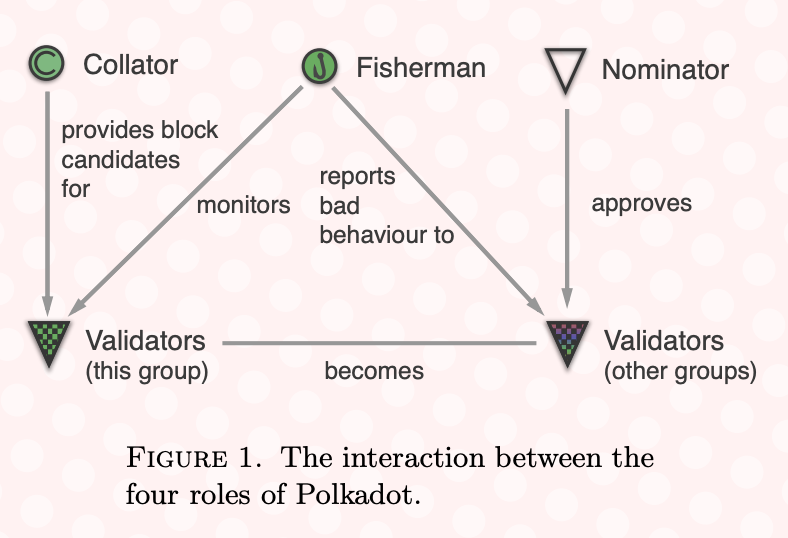
\includegraphics{https://github.com/stakedtechnologies/PolkadotWP/blob/sota/img/Four_Roles.png}
\caption{Figure1}
\end{figure}

\hypertarget{ux30d0ux30eaux30c7ux30fcux30bfux30fc}{%
\subsection{バリデーター}\label{ux30d0ux30eaux30c7ux30fcux30bfux30fc}}

バリデーターはPolkadotネットワークを管理し、新しいブロックを認証する。バリデーターの役割は十分に高額の掛け金がデポジットされているといることに依存している。これは、他の掛け金が賭けられている他のグループから1つ以上のバリデーターを選出し同じように振る舞わせることもできる。なので、バリデーターの掛け金の一部はバリデーターに管理される必要はなく、むしろノミネーターによって管理されていると言える。バリデーターは高い有用性と帯域が必要なクライアントをrelay-cahinで走らせなければならない。それぞれのブロックでノードはノミネートされたparachianで新しいブロックを検証する準備をしなければならない。このプロセスには候補となるブロックの受け取り検証、再発行が含まれている。ノミネーションは決定的であるが、現実的には事前に予測不可能である。バリデーターが全てのparachainのデータベースを全て同期するとは合理的に考えて考えられないので、バリデーターは提案された新しいparachainのブロックを確定する役割をコレイターとして知られる第三者に委託する。

全ての新しいparachainブロックが予定されたバリデーターのサブグループによって適切に検証されたら、バリデーターはrelay-cahinのブロック自体を検証する。この作業にはトランザクションState文字列のアップデート(本質的にはparacahinのアウトプット文字列を他のparacahinのインプット文字列にデータを移すこと。)、検証されたrelaycahinのトランザクションセットのトランザクションを処理すること、最後のparachainの最終変更が含まれるファイナルブロックの承認が含まれている。

バリデーターは私達が選んだコンセンサスアルゴリズムのルール下で彼らの責任を満たさない行動を起こした場合、罰せられる。意図的ではない障害でも、バリデーターの報酬は差し控えられる。繰り返される機能停止は結果的にセキュリティーボンドの減少を招く(バーンを通して)。2重支払いや不正ブロックの共謀などの悪意ある攻撃によって全ての掛け金を失うことになるかもしれない。いくつかの観点で、バリデーターは現在のPoWチェーンにおけるマイニングプールに似ている。

\hypertarget{ux30ceux30dfux30cdux30fcux30bfux30fc}{%
\subsection{ノミネーター}\label{ux30ceux30dfux30cdux30fcux30bfux30fc}}

ノミネーターはバリデーターのセキュリティボンドに貢献するstake-holding
partyである。リスクキャピタルを持ち、そのことによって彼らがネットワークをメンテナンスしている特定のバリデーター(もしくはグループ)を信頼していることを表明すること以外に追加での役割はない。彼らは掛け金の増加、減少に応じて対価を受け取る。次で説明するコレイターと一緒に、ノミネーターはPoWネットワークにおけるマイナーと似ている。

\hypertarget{ux30b3ux30ecux30a4ux30bfux30fc}{%
\subsection{コレイター}\label{ux30b3ux30ecux30a4ux30bfux30fc}}

トランザクションコレイター(略してコレイター)は、バリデーターが正当なparacahinブロックを生成するのをサポートするグループである。彼らは、特定のparachainの``full-node''を持つ。これは、現在のPoWブロックチェーンにてマイナーがしているのと同じように、新しいブロックを監視しトランザクションを実行する為に必要な情報を保持している。普通の状態では、まだ承認されていないブロックを生成するために、トランザクションを照合し実行する。そして、ゼロ知識証明と共にブロックをparachainのブロックを提案する責任をもっているバリデーターに伝播する。

コレイター、ノミネイター、バリデーターの正確な関係は時間とともに変更される可能性が高い。初期は、少数のparacahinとトランザクションが想定されるのでコレイターはバリデーターと密接に働くことを想定している。イニシャルのクライアント実装はparachainのコレイターノードが無条件に正当だとされているparacahinのブロックをrelaycahinのバリデーターに提供するためにRPCを含んでいる。同期されたバージョンの全てのパラチェーンの保管コストが増加するので追加で、そのコストを分散化する経済的インセンティブ設計のあるグループが活動するインフラを作ることが見込まれる。

最終的には、ほぼすべてのトランザクションフィーを回収しようと競争するコレイタープールの存在を期待している。そのようなコレイターは報酬のシェアを目的として特定のバリデーターと一定期間契約を結ぶようになるかもしれない。

代用となる``フリーランス''的なコレイターは
シンプルに、分散化されたノミネイターのプールは掛け金を入れている複数の参加者にバリデーターの仕事をシェアしコーディネートする。これはプールにおけるオープンな参加モデルはさらに分散化したシステムの構築をもたらす。

\hypertarget{ux30d5ux30a3ux30c3ux30b7ux30e3ux30fcux30deux30f3}{%
\subsection{フィッシャーマン}\label{ux30d5ux30a3ux30c3ux30b7ux30e3ux30fcux30deux30f3}}

他の2つの役割とは異なり、フィッシャーマンはブロックの承認プロセスに直接関わってはいない。むしろ、報酬によってモチベートされた``bounty
hunters''として独立している。正確にはフィッシャーマンの存在によってめったに不正行為が起きないことが想定されている。そして、もし不正行為が起こるのであれば悪意ある攻撃というよりもシークレットキーのセキュリティに注意が足りなかったときである。

フィッシャーマンは少なくても1つの掛け金がされている参加者が不正な行為をしたことを時間内に証明することで報酬が得られる。paracahinの場合は、不正行為は同じ鍵で2つの異なるブロックに署名をしたり、不正なブロックを承認するのを手伝ったりすることである。規格外の報酬やセッションのシークレットキーを悪用するのを防ぐために、単一のバリデーターの悪意ある署名メッセージを提供することのベース報酬は最小限に抑えられている。この報酬は他のバリデーターも同様に悪意ある攻撃を仕掛けようとしていた場合、漸近的に増加する。最低でも2/3のバリデーターが善意のある行動をしているというベースセキュリティでは、漸近率は66\%に設定されている。

フィッシャーマンはいくつかの点で必要とされているリソースが相対的に少量で安定性と帯域がそれほど必要ではない現在のブロックチェーンシステムにおける``full
nodes''に似ている。フィッシャーマンは少量の掛け金を支払うという点で異なる。この掛け金はバリデーターの時間とコンピュテーションリソースを奪うという点でシビリアタックを防ぐ効果がある。掛け金はすぐに引き出すことができる。これはおそらく数ドル程度で悪意あるバリデーターの攻撃を防ぐことによって大量の報酬を得ることができる。このセクションではシステム全体の設計像を簡潔に説明する。システムの詳細な説明は章を追って解説する。

\hypertarget{ux30b3ux30f3ux30bbux30f3ux30b5ux30b9}{%
\section{コンセンサス}\label{ux30b3ux30f3ux30bbux30f3ux30b5ux30b9}}

relay-chainでは、Polkadotは正当なブロックが同期性のあるByzantine
faulttolerant
(BFT)アルゴリズムを通して合意される。このアルゴリズムはTendermint
{[}11{]}によってインスパイアされたものである。そして、副次的にHoneyBadgerBFT
{[}14{]}に似通っている。後者は任意の不完全性のある
ネットワークインフラで正常に動作する権威者もしくはバリデーターがいれば効率的でfault-tolerantのコンセンサスを提供する。

proof-of-authority
(PoA)スタイルのネットワークでは、これだけで十分である。しかし、Polkadotは信頼される権威者や3rdパーティーが存在しない完全にOpenでパブリックな環境ネットワークとしてデプロイが可能であるように設計されている。なので私達にはバリデーターを決定し、正直に動くためにインセンティブ設計する必要がある。なので、PoSベースの選考基準を設ける。

\hypertarget{ux639bux3051ux91d1ux3092ux8a3cux660eux3059ux308b}{%
\subsection{掛け金を証明する}\label{ux639bux3051ux91d1ux3092ux8a3cux660eux3059ux308b}}

私達はネットワークに特定のアカウントがいくらの``掛け金''を持っているのかを測る方法があることを想定している。
既存のシステムと比較しやすいように計測する単位を``トークン''とする。この言葉はいくつかの理由で理想的ではない。1つはアカウントに紐付いている値がスカラー値であるとは限らないこと。もう1つは個別のトークンに特有性がないからである。

\begin{figure}
\centering
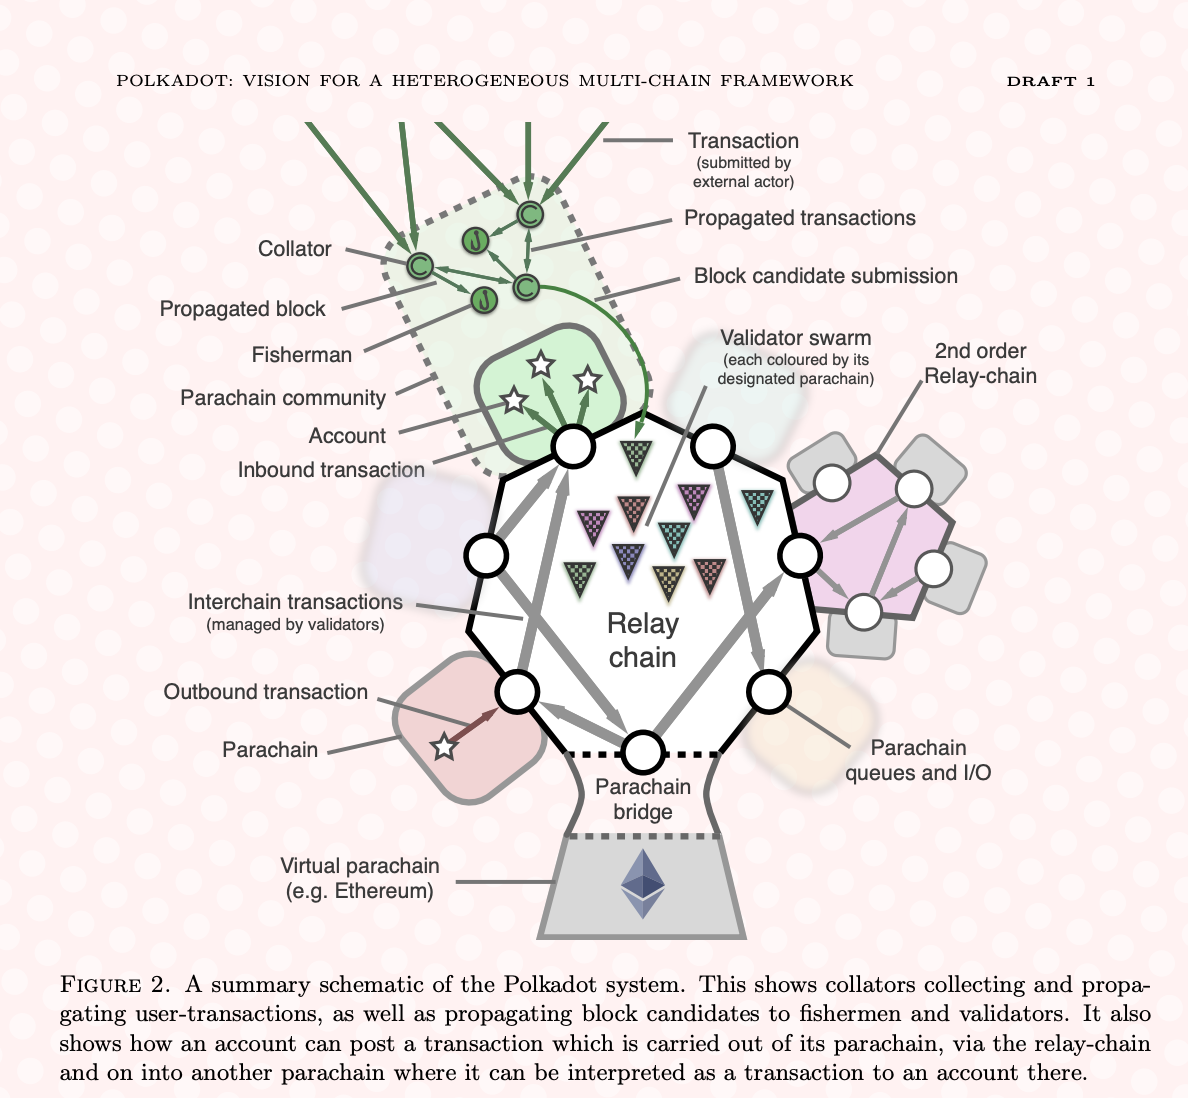
\includegraphics{https://github.com/stakedtechnologies/PolkadotWP/blob/master/img/summary.png}
\caption{Summary}
\end{figure}

私達は、頻度は高くないが(最大でも1日に1回、もしかすると4半期に1回ほど)Nominated
Proof-of-Stake
(NPoS)によってバリデーターは選出されることを想定している。
マネタリーベースの膨張は主にインフレーションをもたらすけれども、全てのトークン保有者が参加権をフェアに持つので、時とともに価値がへるという心配をする必要がない。そのことでコンセンサスメカニズムにおけるトークンホルダーの役割を喜んでこなすようになる。トークンの特定の割合がステーキングプロセスのターゲットとなる。効率的なトークンベースの増加(token
base
expansion)はマーケットベースのメカニズムでこのターゲット値に近づくように調整される。

バリデーターは掛け金によって密接につながっている。バリデーターが掛け金を引き出すことができるのは、バリデーターの責務が終わり時間が経ってからである。(3ヶ月くらい)この長い期間が存在するのは、チェーンのチェックポイントまでバリデーターが将来不正を行った場合罰するためである。報酬額を削減したり、意図的にネットワークを悪化させたり、他のバリデーターに掛け金を渡したりした場合、罰を受けることになる。例えば、バリデーターがフォークした両方のチェーンを承認しようとした場合(しばしばショートレンジアタックと呼ばれる)、後々それが検知され罰せられる。

新しく同期してきたクライアントが間違ったチェーンに騙さないことを確証するために、バリデーターの掛け金整理のタイミングと同じく定期でハードフォークが行われる。これによって最新のチェックポイントブロックハッシュがクライアントに入る。これは今後、``finite
chain
length''やジェネシスブロックを定期的にリセットすることによってうまくいくようになる。

\hypertarget{parachainux3068ux30b3ux30ecux30a4ux30bfux30fc}{%
\subsection{Parachainとコレイター}\label{parachainux3068ux30b3ux30ecux30a4ux30bfux30fc}}

各parachainはrelay-cahinに近いセキュリティー強度を持つ。paracahinのヘッダーはrelay-chainのブロックに格納されており、再編成や2重支払いがないようにしている。これはBitcoinでいうサイドチェーンとマージマイニングと似たセキュリティー保証である。Polkadotではそれに加え、parachainのstate
transactionが正当であるという強い保証を提供する。これは、バリデーターが暗号学的にランダムにサブセットに配属されることを通して行われる。parachainごとにサブセットがあるかもしれなければ、blockごとにサブセットはことなるかもしれない。この設定はparacahinのブロックタイムがrelaycahinのブロックタイムと少なくても同じくらい長いことを示している。この分割の詳しい方法はこの論文の対象外である。しかし、RanDAOに似たcommit-revealフレームワーク、もしくは暗号学的に安全なハッシュ下の各parachainブロックに結合したデータに立脚している可能性が高い。

そのようなバリデーターのサブセットは正当だと保証されたparachainのブロック候補を提供することを要求されている。正当性というのは2つの重要なポイントを含む。1つ目は全てのstate
transitionsが正確に実行され、全ての参照される外部データが最終的に正当であるということ。
2つ目は、that any data which is extrinsic to its candidate, such as
those external transactions, has sufficiently high availability so that
participants are able to download it and execute the block manually.5
Validators may provide only a ``null'' block containing no external
``transactions'' data, but may run the risk of getting a reduced reward
if they do. They work alongside a parachain gossip protocol with
collators---individuals who collate transactions into blocks and provide
a noninteractive, zero-knowledge proof that the block constitutes a
valid child of its parent (and taking any transaction fees for their
trouble).

parachainのプロトコルにチェーン独自のスパム防止方法を搭載する余地を残している。relay-chainにある``compute-resource
metering''もしくは、``transaction
fee''という根本的な概念は存在しない。relaychainプロトコルによってこれらが強制されることもない。(しかし、堅牢なメカニズムの用意されていないparachainをステークホルダーが採用することは起こりえないだろう)これはEthereumのようなチェーンと明確に異っている。(例:シンプルなfeeモデルを持つBitcoinのようなチェーンもしくは、スパム防止モデルは提唱されていないがそれ以外)

Polkadotのrelay-chainそれ自体はEtheruemのようなaccounts、stateチェーンとして存在する可能性が高い。もしかすると、EVMの派生系であるかもしれない。relay-cahinのノードはかなりの処理能力、トランザクションスループットが要求されるので、トランザクションスループットは高いトランザクション手数料とブロックサイズリミットによって最小化されるだろう。

\hypertarget{ux30a4ux30f3ux30bfux30fcux30c1ux30a7ux30fcux30f3ux30b3ux30dfux30e5ux30cbux30b1ux30fcux30b7ux30e7ux30f3}{%
\subsection{インターチェーンコミュニケーション}\label{ux30a4ux30f3ux30bfux30fcux30c1ux30a7ux30fcux30f3ux30b3ux30dfux30e5ux30cbux30b1ux30fcux30b7ux30e7ux30f3}}

Polkadotの重要な最後の要素は、インターチェーンコミュニケーションである。
paracahin間では幾分かのインフォメーションチャネルが存在するので、Polkadotはスケーラブルなマルチチェーンであると私達は考えている。Polkadotの場合、コミュニケーションはできるだけシンプルに設計している。paracahinで処理されるトランザクションは(Chainのロジックによっては)2つ目のparachainもしくは、relay-cahinに発送することができる。商用的なブロックチェーン上の外部トランザクションのように、トランザクションは完全に非同期であり情報をもとの出処に返し継承することはできない。

\begin{figure}
\centering
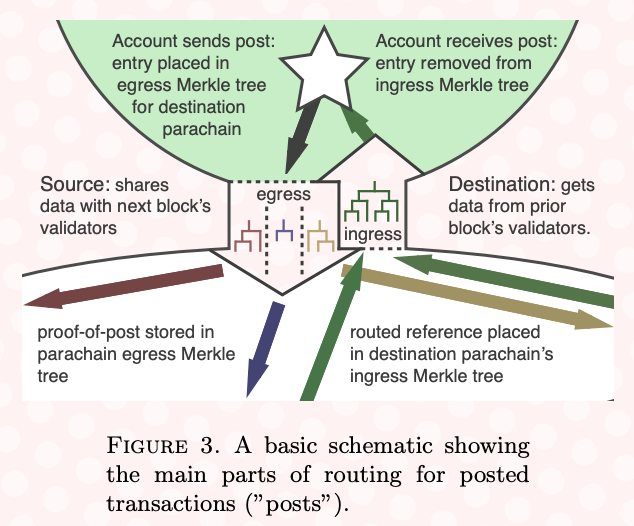
\includegraphics{https://github.com/stakedtechnologies/PolkadotWP/blob/sota/img/transaction.jpg}
\caption{transaction}
\end{figure}

実装の複雑性、リスク、将来のparachainアーキテクチャーの制限を最小化する為に、これらのインターチェーントランザクションは一般的な外部トランザクションと区別することができない。トランザクションはparacahinを認識することができるオリジナルの要素と任意のサイズのアドレスを持つ。BitcoinやEthereumといった現在の一般的なシステムとは異なり、インターチェーントランザクションでは料金が紐づく``決済''はできない。そのような決済は発生源と目的地のparachain間のネゴシエーションロジックを通して管理されなければならない。Ethereum's
Serenityで提案されているシステムはそのようなクロスチェーン決済を管理する簡単な方法である。

インターチェーントランザクションは正確性を保証するMarkle
treeベースの単純な行列メカニズムを使うことによって解決される。1つのparacahinのアウトプット列を目的地のparacahinのインプット列に移動させるのはrelay-cahinのメンテナーの仕事である。その送られたトランザクションはrelay-cahinのトランザクションそれ自体ではなく、relay-chainによって参照される。他のparacahinのトランザクションからparacahinにスパムが送られるのを防ぐために、目的地のインプット列は一番前のブロック列の時よりも大きすぎないようにする必要がある。もしそのインプット列がブロック処理後、大きすぎた場合、それは``仕込まれた''と考えられ、限界値以下に減らさない限り、続くブロックにおいてトランザクションを処理することができなくなる。それらの列はrelay-cahinによって監督され、互いのparachainの状態を監視し合うことができる。なので、不正の目的地にトランザクションが送信された場合、一瞬で報告され目論見は失敗する。(リターンパスが存在しないので、2次トランザクションがこの理由で失敗した場合、オリジナルcallerに報告することができない。他のリカバリー方法が実行される必要がある。)

\hypertarget{polkadotux3068ethereum}{%
\subsection{PolkadotとEthereum}\label{polkadotux3068ethereum}}

Ethereumのチューリング完全性により、お互いにインターオペラビリティを持つ可能性が豊富にあると考えている。少なくても、セキュリティを共有することはできると思う。簡単に言うと、私達はPolkadotからのトランザクションはバリデーターによって署名され、Ethereum上で運用することができ、送信先のコントラクトを起動できるということである。
In the other direction, we foresee the usage of specially formatted logs
(events) coming from a ``break-out contract'' to allow a swift
verification that a particular message should be forwarded.

\hypertarget{polkadotux304bux3089ethereum}{%
\subsection{PolkadotからEthereum}\label{polkadotux304bux3089ethereum}}

Through the choice of a BFT consensus mechanism with validators formed
from a set of stakeholders determined through an approval voting
mechanism, we are able to get a secure consensus with an infrequently
changing and modest number of validators. In a system with a total of
144 validators, a block time of 4 seconds and a 900-block finality
(allowing for malicious behaviour such as double-votes to be reported,
punished and repaired), the validity of a block can reasonably be
considered proven through as little as 97 signatures (twothirds of 144
plus one) and a following 60-minute verification period where no
challenges are deposited. Ethereum is able to host a ``break-in
contract'' which can maintain the 144 signatories and be controlled by
them. Since elliptic curve digital signature (ECDSA) recovery takes only
3,000 gas under the EVM, and since we would likely only want the
validation to happen on a super-majority of validators (rather than full
unanimity), the base cost of Ethereum confirming that an instruction was
properly validated as coming from the Polkadot network would be no more
than 300,000 gas---a mere 6\% of the total block gas limit at 5.5M.
Increasing the number of validators (as would be necessary for dealing
with dozens of chains) inevitably increases this cost, however it is
broadly expected for Ethereum's transaction bandwidth to grow over time
as the technology matures and infrastructure improves. Together with the
fact that not all validators need to be involved (e.g.~only the highest
staked validators may be called upon for such a task) the limits of this
mechanism extend reasonably well. Assuming a daily rotation of such
validators (which is fairly conservative---weekly or even monthly may be
acceptable), then the cost to the network of maintaining this
Ethereum-forwarding bridge would be around 540,000 gas per day or, at
present gas prices, \$45 per year. A basic transaction forwarded alone
over the bridge would cost around \$0.11; additional contract
computation would cost more, of course. By buffering and bundling
transactions together, the break-in authorisation costs can easily be
shared, reducing the cost per transaction substantially; if 20
transactions were required before forwarding, then the cost for
forwarding a basic transaction would fall to around \$0.01. One
interesting, and cheaper, alternative to this multisignature contract
model would be to use threshold signatures in order to achieve the
multi-lateral ownership semantics. While threshold signature schemes for
ECDSA are computationally expensive, those for other schemes such as
Schnorr signatures are very reasonable. Ethereum plans to introduce
primitives which would make such schemes cheap to use in the upcoming
Metropolis hardfork. If such a means were able to be utilised, the gas
costs for forwarding a Polkadot transaction into the Ethereum network
would be dramatically reduced to a near zero overhead over and above the
basic costs for validating the signature and executing the underlying
transaction.

In this model, Polkadot's validator nodes would have to do little other
than sign messages. To get the transactions actually routed onto the
Ethereum network, we assume either validators themselves would also
reside on the Ethereum network or, more likely, that small bounties be
offered to the first actor who forwards the message on to the network
(the bounty could trivially be paid to the transaction originator).

\hypertarget{ethereumux304bux3089polkadot}{%
\subsection{EthereumからPolkadot}\label{ethereumux304bux3089polkadot}}

Getting transactions to be forwarded from Ethereum to Polkadot uses the
simple notion of logs. When an Ethereum contract wishes to dispatch a
transaction to a particular parachain of Polkadot, it need simply call
into a special ``break-out contract''. The break-out contract would take
any payment that may be required and issue a logging instruction so that
its existence may be proven through a Merkle proof and an assertion that
the corresponding block's header is valid and canonical. Of the latter
two conditions, validity is perhaps the most straightforward to prove.
In principle, the only requirement is for each Polkadot node needing the
proof (i.e.~appointed validator nodes) to be running a fully
synchronised instance of a standard Ethereum node. Unfortunately, this
is itself a rather heavy dependency. A more lightweight method would be
to use a simple proof that the header was evaluated correctly through
supplying only the part of Ethereum's state trie needed to properly
execute the transactions in the block and check that the logs (contained
in the block receipt) are valid. Such ``SPV-like''6 proofs may yet
require a substantial amount of information; conveniently, they would
typically not be needed at all: a bond system inside Polkadot would
allow bonded third-parties to submit headers at the risk of losing their
bond should some other third-party (such as a ``fisherman'', see 6.2.3)
provide a proof that the header is invalid (specifically that the state
root or receipt roots were impostors). On a non-finalising PoW network
like Ethereum, the canonicality is impossible to proof conclusively. To
address this, applications that attempt to rely on any kind of
chain-dependent cause-effect wait for a number of ``confirmations'', or
until the dependent transaction is at some particular depth within the
chain. On Ethereum, this depth varies from 1 block for the least
valuable transactions with no known network issues to 1200 blocks as was
the case during the initial Frontier release for exchanges. On the
stable ``Homestead'' network, this figure sits at 120 blocks for most
exchanges, and we would likely take a similar parameter. So we can
imagine our Polkadot-side Ethereuminterface to have some simple
functions: to be able to accept a new header from the Ethereum network
and validate the PoW, to be able to accept some proof that a particular
log was emitted by the Ethereum-side breakout contract for a header of
sufficient depth (and forward the corresponding message within Polkadot)
and finally to be able to accept proofs that a previously accepted but
not-yet-enacted header contains an invalid receipt root. To actually get
the Ethereum header data itself (and any SPV proofs or
validity/canonicality refutations) into the Polkadot network, an
incentivisation for forwarding data is needed. This could be as simple
as a payment (funded from fees collected on the Ethereum side) paid to
anyone able to forward a useful block whose header is valid. Validators
would be called upon to retain information relating to the last few
thousand blocks in order to be able to manage forks, either through some
protocolintrinsic means or through a contract maintained on the relay
chain.

\hypertarget{polkadotux3068bitcoin}{%
\subsection{PolkadotとBitcoin}\label{polkadotux3068bitcoin}}

Bitcoin interoperation presents an interesting challenge for Polkadot: a
so-called ``two-way peg'' would be a useful piece of infrastructure to
have on the side of both networks. However, due to the limitations of
Bitcoin, providing such a peg securely is a non-trivial undertaking.
Delivering a transaction from Bitcoin to Polkadot can in principle be
done with a process similar to that for Ethereum; a ``break-out
address'' controlled in some way by the Polkadot validators could
receive transferred tokens (and data sent alongside them). SPV proofs
could be provided by incentivised oracles and, together with a
confirmation period, a bounty given for identifying non-canonical blocks
implying the transaction has been ``double-spent''. Any tokens then
owned in the ``break-out address'' would then, in principle, be
controlled by those same validators for later dispersal. The problem
however is how the deposits can be securely controlled from a rotating
validator set. Unlike Ethereum which is able to make arbitrary decisions
based upon combinations of signatures, Bitcoin is substantially more
limited, with most clients accepting only multisignature transactions
with a maximum of 3 parties. Extending this to 36, or indeed thousands
as might ultimately be desired, is impossible under the current
protocol. One option is to alter the Bitcoin protocol to enable such
functionality, however so-called ``hard forks'' in the Bitcoin world are
difficult to arrange judging by recent attempts. One possibility is the
use of threshold signatures, cryptographic schemes to allow a singly
identifiable public key to be effectively controlled by multiple secret
``parts'', some or all of which must be utilised to create a valid
signature. Unfortunately, threshold signatures compatible with Bitcoin's
ECDSA are computationally expensive to create and of polynomial
complexity. Other schemes such a Schnorr signatures provide far lower
costs, however the timeline on which they may be introduced into the
Bitcoin protocol is uncertain. Since the ultimate security of the
deposits rests with a number of bonded validators, one other option is
to reduce the multi-signature key-holders to only a heavily bonded
subset of the total validators such that threshold signatures become
feasible (or, at worst, Bitcoin's native multi-signature is possible).
This of course reduces the total amount of bonds that could be deducted
in reparations should the validators behave illegally, however this is a
graceful degradation, simply setting an upper limit of the amount of
funds that can securely run between the two networks (or indeed, on the
\% losses should an attack from the validators succeed). As such we
believe it not unrealistic to place a reasonably secure Bitcoin
interoperability ``virtual parachain'' between the two networks, though
nonetheless a substantial effort with an uncertain timeline and quite
possibly requiring the cooperation of the stakeholders within that
network.

\hypertarget{ux30d7ux30edux30c8ux30b3ux30ebux306eux8a73ux7d30}{%
\section{プロトコルの詳細}\label{ux30d7ux30edux30c8ux30b3ux30ebux306eux8a73ux7d30}}

本プロトコルは大きく3つのパートに分解することができる:コンセンサスメカニズム、パラチェーンインターフェイス、インターチェーン取引ルーティング。

\hypertarget{ux30eaux30ecux30fcux30c1ux30a7ux30fcux30f3ux30aaux30daux30ecux30fcux30b7ux30e7ux30f3}{%
\subsection{リレーチェーンオペレーション}\label{ux30eaux30ecux30fcux30c1ux30a7ux30fcux30f3ux30aaux30daux30ecux30fcux30b7ux30e7ux30f3}}

リレーチェーンはイーサリアムと似たように、ステイトがアドレスをアカウント情報(主に残高や取引回数)にマッピングしたステイトベースのチェーンになるだろう。アカウントをここに置くことには目的が一つある:システムで誰がどれだけのステイクを保持しているかを説明すること。そこには大きな違いはない、しかし:

\begin{itemize}
\tightlist
\item
  コントラクトはトランザクションによって配置することはできない。リレーチェーン上のアプリケーション機能を回避したいという欲求から、契約のパブリックデプロイのサポートをしない。
\item
  計算リソース(ガス)の使用量は計上されない;パブリック使用のための機能のみが直されるため、ガス計上はされなくなる。
\item
  リストに挙げられたコントラクトが自動執行とネットワークメッセージアウトプットをすることを可能にする特殊な機能サポートされる。
\end{itemize}

リレーチェーンにVMがあり、それがEVMをベースにしている場合、単純さを最大化するためにいくつかの変更が必要である。
リレーチェーンにはコンセンサス、バリデーター、パラチェーンコントラクトを行うために、プラットフォーム専用のいくつかの組込みコントラクト(Ethereumの1-4アドレスのような)が存在している。

EVMではない場合、WebAssembly
{[}2{]}(wasm)バックエンドが最も可能性の高い代替手段である。この場合、全体構造は似ているが、埋め込みコントラクトの必要はない。これがEVMのために作られた未熟な言語ではなく汎用言語用であるWasmを使う理由である。

現在のEthereumプロトコルからの全く異なる他のプロトコルの可能性は十分にある。
例えば、EthereumのSerenityのために提案されたように、同一ブロック内で競合しないトランザクションの並列実行を可能にする、簡易的なトランザクション受信フォーマットなど。

これは可能性は低いが、Serenityのような「純粋(Pure)」なチェーンがチェーンの基礎的なプロトコルとしてではなく、Relayチェーンとしてデプロイされるかもしれない。これにより、特定のコントラクトがステイキングトークン残高などを管理することができる。
現時点では、これは追加の複雑さと開発に不確実性を伴う価値がある程の十分なプロトコル簡素化を提供する可能性が低いと感じている。

コンセンサスメカニズム、バリデータセット、バリデーションメカニズムおよびパラチェインを管理するために必要な機能のピースがいくつもある。
これらはモノリシックプロトコルの下で一緒に実装することが可能である。ただし、モジュール性を高めるために、これらをリレーチェーンの「コントラクト」として説明する。

これは、それらが(オブジェクト指向言語のような)オブジェクトであることを意味すると解釈される。リレーチェーンのコンセンサスメカニズムによって管理されているが、必ずしもEVMのようなopcodesでプログラムとして定義されているわけでも、アカウントシステムを通じて個別にアドレス指定可能であるというわけでもない。

\hypertarget{ux30b9ux30c6ux30a4ux30adux30f3ux30b0-ux30b3ux30f3ux30c8ux30e9ux30afux30c8}{%
\subsection{ステイキング
コントラクト}\label{ux30b9ux30c6ux30a4ux30adux30f3ux30b0-ux30b3ux30f3ux30c8ux30e9ux30afux30c8}}

このコントラクトは以下のようにバリデータセットを管理する。

\begin{itemize}
\tightlist
\item
  どのアカウントが現在バリデータであるか(Validators);
\item
  どのアカウントがすぐにバリデータになることができるか(Intentions);
\item
  どのアカウントがバリデータにノミネートするためにステイクしているか(Stashes);
\item
  ステイク量、許容ペイアウト率、アドレス、短期(セッション)アイデンティティを含むそれぞれの特性(Others);
\end{itemize}

それは、アカウントが(その要件と共に)担保付き(bonded)のバリデータになる、ノミネートする、そして既存の担保付きの検証者がこのステータスからエグジットする意思を登録する。またバリデーションと正規化メカニズムのためのメカニズムも含みます。

\hypertarget{ux30b9ux30c6ux30fcux30afux30c8ux30fcux30afux30f3ux306eux6d41ux52d5ux6027}{%
\subsubsection{ステークトークンの流動性}\label{ux30b9ux30c6ux30fcux30afux30c8ux30fcux30afux30f3ux306eux6d41ux52d5ux6027}}

ネットワークセキュリティをステークトークンの全体的な「時価総額」に直結させるため、一般に、できるだけ多くのトータルステーキングトークンをネットワークメンテナンス操作内でステークすることが望ましい。これは、通貨のインフレを通し、収益をバリデータとして参加する人々に配ることによって、容易にインセンティブ設計することができる。しかし、そうすることは一つ問題を提起する:トークンがステークコントラクトでロックされるならば、価格向上を実現するためにどのように十分な流動性を維持できるのか?

これに対する1つの答えは、直接的なデリバティブコントラクトを許可し、ステイクされたトークン上で代替可能(Fungible)なトークンを保護することだ。これは信頼できる方法で手配するのが困難だ。さらに、これらのデリバティブトークンは、異なるユーロ圏の国債が代替可能ではないのと同じ理由で同等に扱うことはできない:原資産が破綻し、価値がなくなる可能性がある。ユーロ圏の政府では、これがデフォルトとなるかもしれない。しかしバリデータがステイクしたトークンの場合、バリデータの悪意を持った行動には処罰が伴う。

私たちは信条を守りながら、最も単純な解決策を選んだ:全てのトークンはステイクされない。つまりは、ある一定の割合(おそらく20%程度)のトークンが強制的に流動性を維持することを意味する。これはセキュリティの観点からは不完全だが、ネットワークのセキュリティに根本的な違いをもたらすことはまずありえない。ステイクの没収による賠償金の80%と、100%のステークの「完璧なケース」との大差はそれほどない。

ステイクされるトークンと流動的なトークンの比率はリバースオークションの仕組みによって案外簡単に決められる。基本的に、バリデーターになりたいトークン保有者はそれぞれ、参加するために必要となる最小支払い率を記載したオファーをステーキング契約に投稿します。各セッションの開始時に(セッションは定期的に、おそらく1時間に1回程度)、各バリデーターのステークとペイアウト率に従ってバリデータースロットが満たされる。これに対する1つの可能なアルゴリズムは、目標総賭け金をスロット数で割った数以下で、その額の半分の下限を下回らない賭け金を表す最低オファーを有するものを選ぶことであろう。スロットを埋めることができない場合は、満たすために下限が何らかの要因で繰り返し引き下げられる。

ステイクしているトークンをアクティブなバリデータにトラストレスにノミネートすることは可能だ。それはバリデータに責任を任せる事になる。ノミネーションは承認投票システムによって行われる。それぞれのノミネーター志望者は、自らの責任の下で彼らがステイクを賭けるのに十分な信頼を置く、一人以上のバリデータをステークコントラクト上に登録することができる。

各セッションで、ノミネーターの掛け金は1人、またはそれ以上のバリデーターに分散される。分散アルゴリズムは、総賭け金がバリデーターセットに最適化する。(The
dispersal algorithm optimises for a set of validators of equivalent
total bonds.)
ノミネーターの賭け金は、バリデーターの責任の下に置かれ、バリデーターの行動応じて利益を得るか、または処罰として減額を受ける。

\hypertarget{ux50b5ux6a29ux306eux6ca1ux53ceux30d0ux30fcux30f3}{%
\subsubsection{債権の没収/バーン}\label{ux50b5ux6a29ux306eux6ca1ux53ceux30d0ux30fcux30f3}}

特定のバリデーターの振る舞いは賭け金に懲罰的な減少をもたらす。賭け金が許容最小額を下回ると、セッションは途中で終了し、別のセッションが開始される。処罰対象のバリデーターの不正行為のリストには以下が含まれる:

\begin{itemize}
\tightlist
\item
  パラチェインブロックの有効性についてコンセンサスを提供できないパラチェイングループの一員である
\item
  無効なパラチェインブロックの有効性について積極的に署名する
\item
  利用可能として以前に投票されたアウトバウンドペイロードを供給することができない
\item
  合意プロセス中に非活動的である
\item
  競合するフォークのリレーチェーンブロックを検証する
\end{itemize}

不正な悪意のある行動のケースによっては、ネットワークの完全性が損なわれ(無効なパラチェインブロックに署名したり、フォークの複数の面を検証したりするなど)、その結果、債権の完全な没収により追い出されることがある。その他の、それほど深刻ではない不正行為(例えば、合意プロセスにおける非活動)または誰の責任か不明瞭である(無効なグループの一部であるなど)場合、代わりに、債権のごく一部の罰金を科されることがある。後者の場合、これはサブグループchurnによって、悪意のあるノードが健全なノードよりより大きな損失を被るようにする。

場合によっては(マルチフォーク検証や無効なサブブロック署名など)、各パラチェインブロックを常に検証するのは面倒な作業になるため、バリデーターがお互いの不正行為を検出することは困難である。ここでは、そのような不正行為を検証し報告するために、検証プロセス外部にある組織の支援を必要とする。その役割を担った存在はそのような活動を報告することで報酬を得る。彼らの「Fisherman(釣り人)」という名前は、そのような稀な報酬に由来している。

これらのケースは通常非常に深刻であるため、いかなる報酬も没収された債券から容易に支払うことができると我々は考えている。一般的に、大規模な再割り当てを試みるのではなく、バーン(つまり、何もしないこと)により再割り当てのバランスを取ることが好ましい。これはトークンの全体的な価値を増加させ、発見に関与する特定の関係者よりもむしろネットワークに対して補償する効果がある。これは主に安全メカニズムとしてのものである。それは大量の報酬を伴ってしまう場合、単一のターゲットに対して報告する極端なインセンティブを与えてしまう事になるかもしれないからだ。

一般的に、報酬はネットワークにとって検証を行うのに十分なほどの大きさである必要がある一方、特定のバリデータに不正行為を強制させるような、組織化されたハッキング攻撃のインセンティブになるほど大きくないことが重要である。

このようにして、報酬は不正行為を行ったバリデータの債権量を超えないようにする必要がある。これは、検証者が故意的に不正行為を行い、自分自身を通報する事で利益を得ないようにするためである。これへの対処法として、バリデータになるのに最低限の賭け金を必要とすることや、ノミネーターに賭け金が少ないバリデーターは不正行為を行うインセンティブが大きい事実を啓蒙するなどがある。

\hypertarget{ux30d1ux30e9ux30c1ux30a7ux30fcux30f3ux30ecux30b8ux30b9ux30c8ux30ea}{%
\subsection{パラチェーンレジストリ}\label{ux30d1ux30e9ux30c1ux30a7ux30fcux30f3ux30ecux30b8ux30b9ux30c8ux30ea}}

各パラチェインはこのレジストリで定義されている。それは比較的単純なデータベースのような構造であり、そして各チェーンに関する静的な情報と動的な情報の両方を保持する。

静的情報には、異なるクラスのパラチェインを区別する手段である検証プロトコルの識別情報とともに、チェーンインデックス(単純な整数)が含まれる。これによって有効な候補を提示するために委任されたバリデータによって正しい検証アルゴリズムが実行される。
最初のPOCでは、新しい検証アルゴリズムをクライアント自体に配置することに重点が置かれ、追加のクラスのチェーンが追加されるたびにプロトコルのハードフォークが事実上必要になる。しかし最終的には、クライアントがハードフォークなしで新しいパラチェインを効果的に処理できるように、厳密かつ効率的な方法で検証アルゴリズムを指定することが可能である。これに対する1つの可能な方法は、WebAssemblyのような確立された、ネイティブにコンパイルされた、プラットフォームに依存しない言語でパラチェイン検証アルゴリズムを指定することである。これが本当に実現可能であるかどうかを判断するには追加の研究が必要だが、もしそうであれば、ハードフォークをしないことにより大きな利点をもたらす可能性がある。

動的情報には、パラチェーンの入力キュー(6.6.で説明)など、グローバルな合意が必要なトランザクションルーティングシステムの側面が含まれている。

レジストリは、全国民投票(referendum)によってのみ追加されたパラチェインを持つことができる。これは内部で管理できるが、より一般的なガバナンス要素のもとでの再利用を促進するために、外部の国民投票コントラクトに入れられる可能性が高くなる。追加チェーンの登録およびその他のあまり正式でないシステムアップグレードのための投票要件(たとえば、必要なクォーラム、大多数の要件)に対するパラメータは、「マスター規約」に記載されるが、少なくとも最初はかなり慣習的な方法に従う。正確な定式化は本研究の範囲外であるが、例えば、システムのステイクの3分の1以上が積極的に投票するという、3分の2のスーパーマジョリティが賢明な出発点となるだろう。

追加の操作には、パラチェーンの一時停止と削除が含まれる。中断は決して起こらないであろうと願っているが、それはパラチェーンのバリデーションシステムに少なくともいくらかの扱いにくい問題があることを保護するセーフガードの役目を担っている。それが必要とされる可能性がある最も顕著な例は、妥当性またはブロックについて合意することができないようにバリデータを導く実装間の重大なコンセンサスの違いである。バリデータは、債権の没収前にそのような問題を発見できるようにするために、複数のクライアント実装を使用することをお勧める。

一時停止は緊急措置であるため、国民投票ではなく動的バリデータ投票によって実行されるだろう。再検証はバリデータからも国民投票からも可能である。

パラチェーンの削除は、国民投票の後に初めて行われ、スタンドアロンチェーンへの秩序ある移行を可能にするため、または他の何らかの合意システムの一部となるためには、かなりの猶予期間が必要である。猶予期間は数ヶ月程度である可能性があり、異なるパラチェーンがそれぞれの必要性に応じて異なる猶予期間を享受できるようにするために、パラチェインレジストリにチェーンごとで設定される可能性がある。

\hypertarget{ux30eaux30ecux30fcux30d6ux30edux30c3ux30afux306eux30b7ux30fcux30eaux30f3ux30b0}{%
\subsection{リレーブロックのシーリング}\label{ux30eaux30ecux30fcux30d6ux30edux30c3ux30afux306eux30b7ux30fcux30eaux30f3ux30b0}}

シーリングとは、本質的には正規化のプロセスを指す。つまり、オリジナルを意味のあるものにマッピングする基本的なデータ変換のことである。POWチェーンの下では、シーリングは事実上マイニングの同義語である。私たちの場合、それは特定のリレーチェーンブロックとそれが表すパラチェーンブロックの有効性、可用性、そして正規性に関するバリデータからの署名されたステートメントの収集を意味する。

基礎となるBFTコンセンサスアルゴリズムのメカニズムの説明は今回の範疇外となる。代わりに、合意形成ステートマシンを想定したプリミティブを使って説明する。最終的には、コアにあるいくつかの有望なBFT合意アルゴリズム(Tangaora
{[}9{]}(Raft {[}16{]}のBFT版)、Tendermint {[}11{]}、HoneyBadgerBFT
{[}14{]})にインスパイアされることを期待している。
このアルゴリズムは、複数のパラチェーンに並行して合意に達する必要があるため、通常のブロックチェーン合意メカニズムとは異なる。一旦合意に達すると、私たちはその合意を反論できない証拠として記録することができ、それは参加者の誰もが提供することができる。我々はまた、処罰に対処する際、プロトコル内の不正行為は一般に不正行為をする参加者を含む小グループにする事により、付随的な被害を最小限に抑えることができると想定している。Tendermint
BFTやオリジナルのSlasherなど、既存のPoSベースのBFTコンセンサススキームは、これらの主張を満たしている。

署名付きステートメントの形式をとる証明は、リレーチェーンブロックのヘッダー、およびその他の特定のフィールド(リレーチェーンのステイトツリーのルートおよびトランザクションツリーのルート)と共に配置される。

シーリングプロセスは、リレーチェーンのブロックと、リレーのコンテンツの一部を構成するパラチェーンのブロックの両方に対応する単一の合意生成メカニズムの下で行われる。パラチェーンは、サブグループによって別々に「コミット」された後に照合されるわけではない。これにより、リレーチェーンの処理がより複雑になるが、システム全体の合意を1段階で完了し、待ち時間を最小限に抑え、以下のルーティング処理に役立つ非常に複雑なデータ可用性の要件を満たすことができる。

各参加者のコンセンサスマシンの状態は、単純な(2次元の)表としてモデル化できる。各参加者(バリデータ)は、各パラチェインブロック候補ならびにリレーチェインブロック候補に関して、他の参加者からの署名付きステートメント(Vote)の形式で一組の情報を有する。情報セットは2つ:

\begin{itemize}
\item
  利用可能性(Availability):このバリデータはこのブロックからのトランザクションの一連の情報を出力していか;故に次のブロックのパラチェイン候補を適切に検証できる。バリデータは1(知られている)か0(まだ知られていない)のどちらかを投票することができる。1を投票した場合、このプロセスの残りの部分についても同様に投票することに一貫する。これに従わない後からの投票は罰の対象となる。
\item
  妥当性(Validity):このパラチェインブロックは有効であり、全ての外部参照データ(例えばトランザクション)は利用可能か。これは、投票しているパラチェーンに割り当てられているバリデータにのみ関係する。彼らは1(有効)、-1(無効)または0(まだ知られていない)のどれかに投票することができる。彼らがゼロでない(non-zero)投票をしたら、このプロセスの残りの部分についても同様に投票することに一貫する。これに従わない後からの投票は罰の対象となる。
\end{itemize}

すべての検証者が投票を提出する必要がある。票は上記の規則によって修飾され、再提出されることがある。合意の進行は、並行して行われる各パラチェインに対する複数の標準的なBFT合意アルゴリズムとしてモデル化することができる。これらは少数の悪意のあるアクターが1つのパラチェイングループに集中することよって潜在的に妨害される。そのため、バックストップを確立するための全体的なコンセンサスが存在し、1つ以上の向こうパラチェインブロックにデッドロックされる最悪のシナリオを防ぐ。

個々のブロックの有効性のための基本的な規則(はバリデータ全体が、正規のリレーから参照されるユニークなパラチェイン候補になることについて合意に達することを可能にする):

\begin{itemize}
\tightlist
\item
  少なくとも3分の2のバリデータがポジティブに投票し、誰もネガティブに投票しないこと。
\item
  3分の1を超えるバリデータが、外に出て行く情報の可用性にポジティブに投票している。
\end{itemize}

正当性について少なくとも1つの正と負の投票がある場合、例外条件が作成され、悪意のある当事者がいるかどうか、または偶然の分岐があるかどうかを判断するためにバリデータのセット全体が投票する必要がある。有効と無効の他に、その両方に対する投票と同等である3番目の種類の投票が許可されている。つまり、ノードには意見の対立がある。これは、ノードの所有者が同意しない複数の実装を実行していることが原因である可能性があり、プロトコルにあいまいさがある可能性があることを示している。

すべての投票が完全なバリデータセットの確認を経た後、負けた側の意見が勝った側の意見の投票のある程度の割合(パラメータ化されるために;最大で半分、おそらくかなりより少ない)を占める場合、それは偶然起こったパラチェーンフォークと考えられ、そのパラチェーンは自動的にコンセンサスプロセスから中断される。さもなければ、それは悪意のある行為であると考えられ、反対意見に投票していた少数派を罰することになる。

結論は、正規性を示す一連の署名である。(The conclusion is a set of
signatures demonstrating
canonicality.)その後、リレーチェーンブロックはシーリングされ、次のブロックをシーリングするプロセスが開始される。

\hypertarget{ux30b7ux30fcux30eaux30f3ux30b0ux30eaux30ecux30fcux30d6ux30edux30c3ux30afux306eux6539ux5584}{%
\subsection{シーリングリレーブロックの改善}\label{ux30b7ux30fcux30eaux30f3ux30b0ux30eaux30ecux30fcux30d6ux30edux30c3ux30afux306eux6539ux5584}}

このシーリング方法はシステムの運用に強力な保証を提供するが、スケールに問題があると考えられている。なぜなら、パラチェインの重要な情報の可用性(Availability)は、バリデータ全体の3分の1以上によって保証されている必要があるためである。そしてこれは、チェーンが追加されるにつれて、すべてのバリデータの責任範囲が増大することを意味する。

オープンコンセンサスネットワーク内のデータの可用性は本質的に未解決の問題であるが、検証ノードにかかるオーバーヘッドを軽減する方法がある。
1つ目の解決策は、バリデータはデータの可用性に対する責任を負うが、実際にデータを保存・通信・複製する必要はないことである。このデータを編集している(あるいはまったく同じ)照合者に関連している可能性がある。
また、(このデータをコンパイルする照合者に関係、または同等であるかもしれない)2次データ格納庫(silos)が、支払いに対する利子/収入の一部を提供しているバリデータ、と可用性を保証するというタスクを管理できる。

しかしながら、これにより一時的なスケーラビリティを得られるが、根本的な問題を解決することにはならない。パラチェーンの追加は、さらなるバリデータを必要とするため、長期的なネットワークリソースの消費量(特に帯域幅の点で)はチェーンの二乗に比例して増加する。

最終的には、合計バリデータ×合計入力情報のバンド幅の基礎制限に手の打ち止めとなるだろう。これは、信頼されていないネットワークが、他の多くのノードにデータストレージのタスクを適切に分配することができないことに起因している。

\hypertarget{ux5f85ux3061ux6642ux9593ux306eux5c0eux5165}{%
\subsubsection{待ち時間の導入}\label{ux5f85ux3061ux6642ux9593ux306eux5c0eux5165}}

この規則を緩和する1つの方法は、即時性の概念を緩和することだ。すぐにではなく、最終的にのみ可用性に投票する33%+
1のバリデータを要求することで、指数関数的データ伝播をより有効に活用し、データ交換のピークを平準化することができる。
(証明されていないが)最も有り得そうな式は次のようになる。

(1)待ち時間=参加者×チェーン ( \emph{latency = participants x chains}
)

現在のモデルでは、システムのサイズはチェーンの数に比例してスケールし、それにより処理が確実に分散される。各チェーンは少なくとも1人のバリデータを必要とし、可用性検証を一定比率のバリデータに固定するため、参加者はチェーンの数が増えるにつれて同様に大きくなる。そしてこれに終始する:

(2)待ち時間= size2 ( \emph{latency = size2} )

つまり、必要な帯域幅と可用性がネットワーク全体で認識されるまでの待ち時間(ファイナライズ前のブロック数とも呼ばれる)は、システムのスケールの2乗に比例して増加する。これは大きな成長要因であり、注目に値するロードブロッカーになる可能性があり、「平坦ではない(non-flat)」パラダイム(リレーチェーンのツリーを介したマルチレベルルーティングを行うため、複数の「Polkadots」を階層的に構成するなど)を実現する。

\hypertarget{ux30d1ux30d6ux30eaux30c3ux30afux53c2ux52a0}{%
\subsubsection{パブリック参加}\label{ux30d1ux30d6ux30eaux30c3ux30afux53c2ux52a0}}

もう1つの可能性のある方向性は、マイクロクレームシステムを通じたプロセスへの一般参加を許可することである。Fishermanと同様に、入手可能性を主張する検証者を監視する外部の存在がありえる。彼らの仕事は、そのような可用性を示すことができないように見える人を見つけることで、他のバリデータにミクロの苦情を申し立てることができる。システムをほとんど役に立たなくするようなシビル(sybil)攻撃を軽減するために、電力またはステークボンドを使用することができる。

\hypertarget{ux53efux7528ux6027ux306eux4fddux8a3cux4eba}{%
\subsubsection{可用性の保証人}\label{ux53efux7528ux6027ux306eux4fddux8a3cux4eba}}

最終的な方法は、「可用性保証者」として2組目のステイク済みバリデータをノミネートすることである。これらは通常のバリデータと同じように結合され、同じセットから取られることさえ可能だ(少なくともセッションごとに、長期間にわたって選択される)。通常のバリデータとは異なり、パラチェインを切り替えるのではなく、重要なインターチェーンデータの可用性を証明するために単一のグループを形成する。

これには、参加者とチェーン間の同等性が緩和されるという利点がある。本質的に、チェーンは(元のチェーンバリデータセットと一緒に)成長することができるが、参加者、特にデータ可用性テストに参加している参加者は、最低限の準線形(sub-linear)に留まる可能性がある。

\hypertarget{ux7167ux5408ux8005collatorux306eux8a2dux5b9a}{%
\subsubsection{照合者(Collat​​or)の設定}\label{ux7167ux5408ux8005collatorux306eux8a2dux5b9a}}

このシステムの重要な側面の1つは、どのパラチェイン内にもブロックを作成するための健全なコレクターの選択が行われていることを確認することである。単一の照合者がパラチェインを支配していた場合、外部データの可用性が不足する可能性はそれほど明白ではないため、いくつかの攻撃がより実行可能となる。

1つの選択肢は、擬似ランダムメカニズムでパラチェインブロックを人為的に重み付けすることにより、照合者の多様化を行うことだ。第一に、合意メカニズムの一部として、バリデーターが「より重い」と判断したパラチェインブロック候補を支持することを要求する。同様に、バリデータが最も重いブロックを提案することを動機付ける必要がある
-
これは彼らの報酬の一部を候補の重さに比例させることを通してなされるかもしれない。

照合者が彼らの候補が勝利候補として選択される合理的公平な機会が与えられることを確実にするために、パラチェインブロック候補の具体的な重みを各照合者のランダム関数で決定する。たとえば、照合者のアドレスと、作成されているブロックのポイントの近くで決定される暗号的に安全な疑似乱数の間のXOR距離の測定(概念的な「勝利チケット」)。これにより、各照合者(より具体的には各照合者のアドレス)に、候補者ブロックが他のすべての候補者よりも「勝つ」というランダムなチャンスが与えられる。

1人の照合者が勝利チケットに近いアドレスを「マイニング」してそのブロックをお気に入りにするというシビル攻撃を防ぐために、照合者のアドレスに慣性(inertia)を導入する。これは、アドレスに基準金額の資金があることを要求するのと同じくらい簡単かもしれない。よりエレガントなアプローチは、問題のアドレスに溜まっている資金の量で、勝利チケットの近くに重みを付けることだ。モデリングはまだ行われていないが、このメカニズムによって、ごくわずかなステイク者でも照合者として貢献できる可能性がある。

\hypertarget{ux592aux308aux3059ux304eux305foverweightux30d6ux30edux30c3ux30af}{%
\subsubsection{太りすぎた(Overweight)ブロック}\label{ux592aux308aux3059ux304eux305foverweightux30d6ux30edux30c3ux30af}}

バリデータセットが危険に晒されている場合、有効ではあるが実行と検証に時間がかかるブロックを作成して提案する可能性がある。バリデータグループは、ショートカットを可能にする特定の情報が既に知られていない限り、実行するのに非常に長い時間がかかるブロックを合理的に形成できるので問題となる。
1人の照合者がその情報を知っていれば、他の古いブロック処理をしている人に対し、自分の候補者を受け入れさせることに明らかなアドバンテージとなる。これらのブロックを太りすぎ(Overweight)と呼ぶ。

追加の注意点はあるが、これらのブロックを送信して検証するバリデータに対する保護は、無効なブロックとほぼ同じように考えられる。ブロックを実行するのにかかる時間は主観的であり、投票の最終結果は不正行為については、基本的に3つに分類される。
1つの可能性は、ブロックが明らかに太りすぎではないということだ -
この場合、3分の2以上がブロックをある限度内で実行できると宣言している(例えば、ブロック間の合計許容時間の50%)。2つ目は、ブロックが確実に太り過ぎであるということだ。これは、3分の2以上が、制限内でブロックを実行できないと宣言した場合。
最後の可能性はバリデータ間の意見が半分に割れることだ。この場合、我々は何らかに比例した罰をすることを選ぶかもしれない。

バリデータがいつ太りすぎのブロックを提案している可能性があるかをバリデータが確実に予測できるようにするには、ブロックごとに自分のパフォーマンスに関する情報を公開するように要求することを勧める。十分な期間にわたって、彼らが判断しようとしている仲間と比較して彼らの処理速度をプロファイルすることを可能にするはずだ。

\hypertarget{ux30b3ux30ecux30fcux30bfux30fcux4fddux967a}{%
\subsubsection{コレーター保険}\label{ux30b3ux30ecux30fcux30bfux30fcux4fddux967a}}

バリデータに関して1つの問題が残っている:PoWネットワークとは異なり、有効性について照合者のブロックをチェックするために、彼らは実際にその中のトランザクションを実行しなければならない。悪意のある照合者は、無効な、または太りすぎのブロックをバリデータに供給することができ、グリーフ(リソースの無駄遣い)を引き起こし、潜在的にかなりの機会損失を強制する。

これを軽減するために、バリデータ側で単純な戦略を提案する。第一に、バリデータに送られるパラチェインブロック候補は資金があるリレーチェーン口座から署名されなければならない。そうでない場合、バリデータはすぐにそれを削除する必要がある。第二に、そのような候補者は、ある上限までの口座内の資金の額、過去に丁寧に提案した過去のブロック数までの組み合わせ(例えば、乗算)によって優先的に順序付けされるべきである。
)、および前述のように当選チケットへの近接係数。上限は、無効なブロックを送信した場合にバリデータに支払われる懲罰的損害賠償と同じでなければならない。

無効または過重のブロック候補を検証者に送信することを照合者にさせないために、検証者は不正な照合者の口座にある資金の一部または全部を不正な検証者に移すという影響で、不正行為を主張する違反ブロックを含むトランザクションを次のブロックに入れることができる。このタイプの取引は、罰金の前に照合者が資金を取り出すことをできないようにするために、他の取引を前倒しで実行する。損害賠償として譲渡される資金の額は、まだモデル化されていない動的パラメータだが、生じたグリーフのレベルを反映するためのバリデータブロック報酬の割合となる可能性がある。悪意のある検証者が照合者の資金を勝手に没収するのを防ぐために、照合者は小額の入金の見返りにランダムに選択された検証者の陪審員による検証者の決定に上訴することができる。彼らがバリデータの支持を得た場合、デポジットは彼らによって消費される。そうでなければ、保証金は返却され、バリデーターは罰金を科される(バリデーターははるかにアーチ型の位置にあるので、罰金はかなり多額になるだろう)。

\hypertarget{ux30c1ux30a7ux30fcux30f3ux9593ux30c8ux30e9ux30f3ux30b6ux30afux30b7ux30e7ux30f3ux30ebux30fcux30c6ux30a3ux30f3ux30b0}{%
\subsection{チェーン間トランザクションルーティング}\label{ux30c1ux30a7ux30fcux30f3ux9593ux30c8ux30e9ux30f3ux30b6ux30afux30b7ux30e7ux30f3ux30ebux30fcux30c6ux30a3ux30f3ux30b0}}

チェーン間トランザクションルーティングは、リレーチェーンとそのバリデータの重要なメンテナンスタスクの1つである。これは、転記されたトランザクションが、ある信頼要件を必要とせずに、ソースパラチェーンからの希望する出力から他のデスティネーションパラチェーンの非交渉入力になる方法を決定するロジックである。

私たちは上の言葉を慎重に選ぶ。特に、この投稿を明示的に承認したために、ソースパラチェイン内にトランザクションがあったことを要求しない。私たちのモデルに課せられる唯一の制約は、パラチェインが全体のブロック処理出力の一部としてパッケージされ、ブロックの実行の結果であるポストを提供しなければならないということだ。

これらのポストは複数のFIFOキューとして構成されている。リストの数はルーティングベースと呼ばれ、16前後になる場合がある。特に、この数は、マルチフェーズルーティングに頼らなくてもサポートできるパラチェインの数を表す。当初、Polkadotはこの種の直接ルーティングをサポートするが、最初の一連のパラチェーンをはるかに超えてスケ​​ールアウトする手段として、1つの可能な多相ルーティングプロセス(「ハイパールーティング」)の概要を説明する。

すべての参加者が次の2つのブロックn、n +
1のサブグループを知っていると仮定する。要約すると、ルーティングシステムは次の段階に従う。

\begin{itemize}
\tightlist
\item
  CollatorS : Contact members of V alidators{[}n{]}{[}S{]}
\item
  CollatorS: FOR EACH subgroup s: ensure at least 1 member of V
  alidators{[}n{]}{[}s{]} in contact
\item
  CollatorS : FOR EACH subgroup s: assume egress{[}n −
  1{]}{[}s{]}{[}S{]} is available (all incoming post data to `S` from
  last block)
\item
  CollatorS: Compose block candidate b for S: (b.header, b.ext, b.proof,
  b.receipt, b.egress)
\item
  CollatorS : Send proof information proof{[}S{]} = (b.header, b.ext,
  b.proof, b.receipt) to V alidators{[}n{]}{[}S{]}
\item
  CollatorS : Ensure external transaction data b.ext is made available
  to other collators and validators
\item
  CollatorS : FOR EACH subgroup s: Send egress information
  egress{[}n{]}{[}S{]}{[}s{]} = (b.header, b.receipt, b.egress{[}s{]})
  to the re- ceiving sub-group's members of next block V alidators{[}n +
  1{]}{[}s{]}
\item
  V alidatorV : Pre-connect all same-set members for next block: let N =
  Chain{[}n + 1{]}{[}V {]}; connect all validators v such that Chain{[}n
  + 1{]}{[}v{]} = N
\item
  V alidatorV : Collate all data ingress for this block: FOR EACH
  subgroup s: Retrieve egress{[}n − 1{]}{[}s{]}{[}Chain{[}n{]}{[}V
  {]}{]}, get from other val- idators v such that Chain{[}n{]}{[}v{]} =
  Chain{[}n{]}{[}V{]}.Possibly going via randomly selected other val-
  idators for proof of attempt.
\item
  V alidatorV : Accept candidate proofs for this block
  proof{[}Chain{[}n{]}{[}V {]}{]}. Vote block validity
\item
  V alidatorV : Accept candidate egress data for next block: FOR EACH
  subgroup s, accept egress{[}n{]}{[}s{]}{[}N {]}. Vote block egress
  availability; re- publish among interested validators v such that
  Chain{[}n + 1{]}{[}v{]} = Chain{[}n + 1{]}{[}V {]}. • V alidatorV :
  UNTIL CONSENSUS
\end{itemize}

ここで、egress {[}n{]} {[}from{]} {[}to{]}は、ブロック番号
'n'のparachain 'from'からparachain
'to'への投稿に対する現在の出力キュー情報である。
Collat​​orSは、パラチェインSのCollator。Validators {[}n{]}
{[}s{]}は、ブロック番号nのパラチェインsのバリデータのセット。逆に、Chain
{[}n{]}
{[}v{]}はバリデータvがブロック番号nに割り当てられているパラチェイン。
block.egress
{[}to{]}は、宛先parachainがtoである、あるparachainブロックブロックからの投稿の出力キュー。

照合者は、自分のブロックが正規になったことに基づいて料金を徴収するため、次のブロックの送信先ごとに、サブグループのメンバーに現在のブロックからの出力キューが通知される。バリデータは(パラチェイン)ブロックについてコンセンサスを形成することのみを奨励されている。原則として、バリデータは照合者と忠誠を尽くし、他の照合者のブロックが標準的になる可能性を減らすために共謀することができるが、これはパラチェインのバリデータをランダムに選択するため整理するのが困難であり、合意プロセスを妨げるパラチェインブロックに対して支払うべき料金の減少で擁護される可能性がある。

\hypertarget{ux30d7ux30edux30c8ux30b3ux30ebux306eux5b9fux7528ux6027}{%
\section{プロトコルの実用性}\label{ux30d7ux30edux30c8ux30b3ux30ebux306eux5b9fux7528ux6027}}

\hypertarget{ux30c1ux30a7ux30fcux30f3ux9593ux306eux30c8ux30e9ux30f3ux30b6ux30afux30b7ux30e7ux30f3ux652fux6255ux3044}{%
\subsection{チェーン間のトランザクション支払い}\label{ux30c1ux30a7ux30fcux30f3ux9593ux306eux30c8ux30e9ux30f3ux30b6ux30afux30b7ux30e7ux30f3ux652fux6255ux3044}}

Ethereumのガスのような、全体的な計算リソースの必要性を無くすフレームワークによって、大きな自由と単純さが得られる一方で、これは重要な問題を提起する:いかにパラチェインAはパラチェインBによる計算の強制を防ぐのか。
1つのチェーンがトランザクション''データ''を別のチェーンにスパムすることはトランザクションポスト入力キューバッファ(transaction-post
ingress queue
buffers)によって防ぐことができるが、トランザクション''処理''のスパムを防ぐためのメカニズムはプロトコルによって提供されていない。

これはより高レベルの問題である。チェインは送られてくるトランザクションPOSTデータに任意のセマンティクスデータを付けることができるため、料金は計算を開始する前に確実に支払われる必要がある。
Ethereum
Serenityによって支持されたモデルと同様に、一定量の処理リソースの提供と引き換えに、バリデータに保証された支払いを可能にする''break-in''コントラクトをパラチェイン内で想像することができる。これらのリソースは、ガスのようなもので測定されるかもしれないが、主観的な実行時間やBitcoinのようなフラットフィーモデルのような、まったく新しいモデルである可能性もある。

``break-in''コントラクトで認識されている価値のメカニズムが何か、オフチェーンの呼び出し元からは想定できないため、これ単体ではそれほど役に立たない。しかし、ソースチェーンに二次的な''break-out''コントラクトがあると想像できる。この2つのコントラクトは互いに橋渡しをし、お互いを認識し、価値の同等性を提供する(それぞれが持つステイクトークンがbalance-of-paymentを行うのに使われるかもしれない)。他のそのようなチェーンにCallすることは、このブリッジを介してプロキシを行うことを意味する。これは、目的地のパラチェインに必要な計算リソースを支払うために、チェーン間の価値の移転を交渉するための手段を提供する。

\hypertarget{ux8ffdux52a0ux306eux30c1ux30a7ux30fcux30f3}{%
\subsection{追加のチェーン}\label{ux8ffdux52a0ux306eux30c1ux30a7ux30fcux30f3}}

パラチェインの追加は比較的安価な操作だが無料ではない。パラチェインが多いほど、パラチェインごとのバリデータが少なくなり、最終的には平均賭け金量が少なくなったバリデータが多くなる。パラチェインを攻撃するためのコスト減少問題は、Fishermanの役割によって軽減されるが、成長しているバリデータセットは、元となるコンセンサスメカニズムにより長い待ち時間を発生させる。さらに、各パラチェインは、過度に煩わしい検証アルゴリズムを使用して検証者を苦しめる可能性をもたらす。

よって、バリデータやステイキング
しているコミュニティのために、新しいパラチェインを追加することに値段が付いている。この「チェーン市場」では、次のいずれかが追加される可能性がある:

-(ステーキングトークンのロックアップやバーンの観点から)メンバーになるために拠出金の支払いがゼロになっている一部のチェーン(例:コンソーシアムチェーン、Dogeチェーン、アプリ固有のチェーン)。
-
他では手に入れることが困難な特定の機能(機密性、内部スケーラビリティ、サービスの結びつきなど)を追加することにより、ネットワークに固有の価値を提供するチェーン。

基本的には、ステイク保持者のコミュニティに子供チェーンを追加してもらうため、インセンティブ(例:金銭・機能的なチェーンをリレーに追加したいという意思)を与える必要がある。
追加された新しいチェーンに対しての削除通知の期間は非常に短い。これにより、中長期的な全体の価値へのリスクなしに、新しいチェーンを実験的に追加することができるようになることを想定している。

\hypertarget{ux7d50ux3073}{%
\section{結び}\label{ux7d50ux3073}}

ここまで、スケーラブルで特定の既存ブロックチェーンネットワークと下位互換性がある、異多種を含むマルチチェーンプロトコルをいかに実現するかを概説した。そのようなプロトコルの下で参加者は、例外的に自由に拡張することができる、標準的なブロックチェーン設計から来る既存のユーザにも特に費用が要さない、システムを創り上げるために自己関心で行動する。
すでに参加者の性質、参加者の経済的インセンティブ、参加するために必要なプロセスなど、それに伴うアーキテクチャの大まかな概要を示した。基本デザインを分析し、その長所と短所について説明した。これからの我々の方向は、これらの短所・制限を減らし、完全にスケーラブルなブロックチェーンソリューションを生み出すこと目指す。

\hypertarget{ux6b20ux3051ux3066ux3044ux308bux8cc7ux6599ux3068ux672aux89e3ux6c7aux306eux8ceaux554f}{%
\subsection{欠けている資料と未解決の質問}\label{ux6b20ux3051ux3066ux3044ux308bux8cc7ux6599ux3068ux672aux89e3ux6c7aux306eux8ceaux554f}}

ネットワークフォークの可能性は、プロトコルの異なる実装によっては常に存在する。そのような例外的な状態からの回復についての議論はまだ行われていない。ネットワークには必ずゼロではないファイナライズ期間があることを考えると、リレーチェーンのフォークから回復することは大きな問題ではないはずだが、合意プロトコルへの慎重な統合が必要になる。

債券の没収と通報による報酬の提供は、まだ深く検討されていない。現時点では、報酬はwiner-takes-allを元に提供されると想定している。これは、Fishermanにとって最良のインセンティブモデルではないかもしれない。短期間のコミット啓示プロセスでは、多くのFishermanが報酬のより公平な配分を主張することができるが、そのプロセスは不正行為の発見にさらなる遅れをもたらす可能性がある。

\hypertarget{ux8b1dux8f9e}{%
\subsection{謝辞}\label{ux8b1dux8f9e}}

これを漠然とした形にするのを手伝ってくれたすべての校正読者に感謝します。特に、Peter
Czaban、Bjo ̈rn Wagner、Ken Kappler、Robert Habermeier、Vitalik
Buterin、Reto Trinkler、Jack Petersson。特に Marek Kotewicz氏とAeron
Buchanan氏は特別な感謝が必要ですね。他にもアイデアを提供してくれたすべての人々と、その始まりに感謝します。そして、その過程での彼らの助けを他の皆に感謝します。すべての誤りは私の責任とします。

合意アルゴリズムの初期調査を含むこの研究の一部は、Innovate
UKプログラムの下で、英国政府によって部分的に資金提供されました。

\hypertarget{appendix-a.-ux6a5fux80fdux30b3ux30f3ux30ddux30fcux30cdux30f3ux30c8}{%
\section{APPENDIX A.
機能コンポーネント}\label{appendix-a.-ux6a5fux80fdux30b3ux30f3ux30ddux30fcux30cdux30f3ux30c8}}

ハイレベルから見ると、Parity Polkadot
Platformスタックには多数の機能コンポーネントがあり、それの完成にはかなりの量の研究開発が必要になる。
コンポーネントには既存の他コンポーネントに依存しているものも、独立しているものもある。プラットフォームが正しく機能するために非常に重要なものもあれば、あったほうがいい(nice-to-haves)ものもある。未確定の複雑さでまだ実行可能と見なされていないものや、比較的簡単なものもある。ここでは、それらのコンポーネントをできる限り多く、それらが開発ロードマップのどこに収まるかをリストする。

\begin{itemize}
\tightlist
\item
  ネットワーキングサブシステム(Networking
  subsystem):ピアネットワークが形成され維持される手段。初期のシステムでは、既存のp2pネットワークライブラリ(devp2p)に単純な変更をするだけで十分である。ただし、ネットワークが成長するにつれて、ネットワークtopologyがますます構造化され、最適なデータロジスティクスが可能になるようにするには、追加の研究開発が必要になる。最終的なデプロイのために、libp2p、devp2p、およびGNUnetの適応は最初に考慮されるべき問題だ。要件が満たされそうにない場合は、新しいプロトコルを検討する必要がある。
\item
  コンセンサスメカニズム(Consensus
  mechanism):Proof-of-authorityコンセンサスメカニズム:豊富なバリデータステートメントをサポートし、部分的なステートメントの主観的な受領に基づき、複数の独立したアイテムを一連の単一プロセスの下で合意を可能にする。このメカニズムは、悪意のあるバリデータを棄却するための不正行為の証明を許可する必要がありますが、ステーキングメカニズムを含む必要はありません。相当量の研究とプロトタイピングがこのコンポーネントの開発に必要。
\item
  Proof-of-stakeチェイン:合意メカニズムをPOS領域に拡張する。このモジュールには、ステイクトークン、検証者プールへの出入り管理、検証報酬を決定する市場メカニズム、ノミネーション承認投票メカニズムのファイナライズ、および債券の没収、削除の管理が含まれる。まだ最終的な開発の前に相当量の研究とプロトタイプが必要。
\item
  Parachainの実装(Parachain
  Implementation):最初のParachainの実装は、Bitcoinや(より豊富なトランザクションを提供するため)Ethereumなどの既存のブロックチェーンプロトコルに大きく基づく可能性がある。これには、POSチェーンとの統合が含まれ、パラチェインが独自の内部コンセンサスメカニズムなしに合意を獲得することを可能にする。
\item
  トランザクション処理サブシステム(Transaction processing
  subsystem):パラチェインとリレーチェーンの進化により、トランザクションの送信、受信、伝播が可能になる。これには、ネットワーク層でのトランザクションキューイングと最適化されたトランザクションルーティングの設計が含まれる。
  トランザクションルーティングサブシステム:これはリレーチェーンにさらなる複雑性をもたらす。まずは、パラチェーンに取引可能性(transactability)を追加することが必要になる。それに続き、リレーチェーンにハードコードされた2つのパラチェインで、それは入力/出力キューの管理を含む。最終的に、ネットワークプロトコルとともに有向トランザクション伝播(directed
  transaction
  propagation)の手段へと発展し、独立したパラチェイン照合者が興味のないトランザクションに過度にさらされないようにする。
\item
  リレーチェーン(Relay
  chain):これはリレーチェーン(relay-chain)の最終段階で、パラチェーンの動的な追加、削除、緊急停止、不正行為の報告、そして「Fisherman」機能の実装を含みます。
\item
  独立した照合者(Independent
  collators):これは代替のチェーン固有の照合者機能の提供である。証明作成(照合者用)、パラチェインの不正行為検知(fisherman用)、検証機能(検証者用)が含まれる。また、2人が発見して通信するために必要な追加のネットワークも含まれる。
\item
  ネットワークダイナミクスのモデル化と研究:このプロトコルの全体的なダイナミクスは徹底的に研究されるべきである。これは、オフラインのネットワークモデリングと、シミュレートされたノードを介した実証的根拠の両方によって起こり得る。後者はリレーチェーンに依存しており、ノードが照合者のために彼らのアクションに関する詳細なレポートを中央ハブに提出することを可能にする、構造化されたロギングプロトコルの開発を含む。
\item
  ネットワークインテリジェンス:複雑な分散型マルチパーティネットワークとして、\url{http://ethstats.net}
  に似たネットワークインテリジェンスハブがネットワーク全体のライフサインを監視し、潜在的な破壊行動にフラグを立てるために必要である。最大の効率を得るためには、構造化ロギングを使用し、このデータをリアルタイムで生成、および視覚化する必要がある。そしてそれは、リレーチェーンが合理的な完全状態であることに依存する。
\item
  情報公開プラットフォーム(Information publication
  platform):これは、そのブロックチェーンに関連するデータを公開するためのメカニズムであり、事実上、分散型コンテンツ発見ネットワークを意味する。最初は基本的なP2P検索で処理できるが、可用性が重要であるため、デプロイにはより構造化された堅牢なソリューションが必要になるだろう。
  IPFS統合は、これらの目標を達成するための最も賢明な手段かもしれない。
\item
  Javascriptインタラクションバインディング:ネットワークとインタラクトするための主な手段は、おそらくEthereumの例に従うだろう。そのため、高品質のJavascriptバインディングが重要である。私たちのバインディングは、リレーチェーンと最初のパラチェインとの相互作用をカバーし、それ自体はそれらに依存する。
\item
  ガバナンス:当初、これはハードフォーク、ソフトフォーク、およびプロトコルの再パラメータ化などの例外的なイベントを管理するためのリレーチェーン上のメタプロトコルになる。それはコンフリクトを管理し、ライブロック(live-locks)を防ぐための近代的な構造である。最終的に、これは通常、ハードフォークにしかできない変更を実行することができる完全なメタプロトコル層になるかもしれない。リレーチェーンが必要。
\item
  インタラクションプラットフォーム:ノーマルユーザーが、賭けプロセスへの参加、投票、トークン転送、ノミネーター、バリデータ、Fisherman、または照合者になるなどの一般的なタスクを容易にするための、最小限の機能を用いてシステムと対話できるプラットフォーム。機能的なリレーチェーンを持つことに依存する。
\item
  ライトクライアント:開発されるリレーチェーンとあらゆるパラチェインのためのライトクライアント技術。これにより、クライアントは、トラストレスに、ストレージや帯域幅をほとんど必要とせず、チェーン上のアクティビティに関する情報を入手できるようになる。リレーチェーンに依存する。
\item
  パラチェイン
  UI:マルチチェーン、マルチトークンのウォレットとID管理システム。ライトクライアント技術とインタラクションプラットフォームが必要。これは初期のネットワーク配置には必要ない。
\item
  チェーン上のDappサービス:初期のパラチェーンにデプロイする必要があるさまざまなサービス(API、名前、自然言語の仕様、コードなどのための登録ハブなど)。これはパラチェインによるが、初期のネットワーク配置には必ずしも必要ではない。
\item
  アプリケーション開発ツール:開発者を支援するために必要なさまざまなソフトウェアが含まれている。例としては、コンパイラ、キー管理ツール、データアーカイバ、VMシミュレータなど、他にもたくさん存在している。これらは必要に応じて開発する必要があり、そのようなツールの必要性を最小限に抑えるために、テクノロジは部分的に選択される。またその多くは厳密には必要とされていない。
\item
  パラチェインとしてのEthereum(Ethereum-as-a-parachain):Ethereumから/へのトラストフリーのブリッジにより、投稿されたトランザクションがパラチェーンからEthereumへルーティングされ(他の外部からのトランザクションと同じ扱い)、Ethereum上のコントラクトがパラチェーンとその内部のアカウントにトランザクションを送れるようにする。
  最初に、これは実現可能性を確かめるためにモデル化され、合意プロセスに必要なバリデータの数、それが依存している要素に基づき、構造上の制限を確定する必要がある。これに続き、Proof-of-conceptを構築することができ、最終的な開発はリレーチェーン自体に依存する。
\item
  Bitcoin-RPC互換レイヤー(Bitcoin-RPC compatibility
  layer):リレーチェーン用の単純なRPC互換レイヤーで、そのプロトコルを使用して既に構築されているインフラをPolkadotと相互運用可能にし、サポートの手間を最小限に抑える。リレーチェーンを必要とする挑戦的な目標。
\item
  Web
  2.0バインディング:Polkadotインフラをレガシーシステムで使用しやすくするために、共通のWeb
  2.0テクノロジスタックにバインドします。最初のパラチェインと公開されるチェーン上のインフラに依存する挑戦的な目標。
\item
  zk-SNARKパラチェインの例:zk-SNARKを利用して、トランザクションの身元を確実に秘匿にするパラチェイン。挑戦的目標はリレーチェーンに依存します。
\item
  暗号化されたパラチェインの例:状態の各項目を暗号化された、および署名された状態に保つパラチェイン。これらは、その中のデータの検査と修正に対するアクセス制御の執行を確実にし、商業的に規制された業務が必要に応じて順応することを可能にする。元となる情報が晒されることなく、Polkadotバリデータがある程度の状態遷移の正しさを保証することを可能にするためのProof-of-authorityメカニズムを含む。リレーチェーンに応じた挑戦的目標。
\item
  トラストフリーなBitcoinブリッジ:トラストフリーBitcoinの「双方向ペグ(two-way-peg)」機能。これは、おそらく、閾値署名、あるいはSPV証明&専門のFishermanと一緒にm
  / n(n of
  m)マルチ署名Bitcoinアカウントを使用するだろう。開発は初期の実現可能性分析に基づいており、好ましい結果が得れている。この機能をサポートするには、Bitcoinプロトコルに/から追加機能/ロック解除が必要。
\item
  抽象的/低レベルの分散型アプリケーション(Abstract/low-level
  decentralized
  application):トラストフリートークン交換、資産追跡インフラ、クラウドセールスインフラ。
\item
  コントラクト言語:プロジェクトに絶対必要な部分ではないが、挑戦的な目標だといえる。チュートリアル、ガイドライン、および教育ツールとともに安全なコントラクト言語が用意されるだろう。それはオリジナルSolidity言語のビジョンに従い、形式的な証明をする手段となるか、あるいは関数型言語や条件付き言語のような重大なプロセスエラーを最小にするプログラミングパラダイムに基づいているかもしれない。
\item
  IDE:コントラクト言語に基づき、これはパラチェイン上でのコントラクトの編集、コラボレーション、発行およびデバッグを容易にする。さらなる挑戦的目標である。
\end{itemize}

\hypertarget{appendix-b.-frequently-asked-questions}{%
\section{APPENDIX B. FREQUENTLY ASKED
QUESTIONS}\label{appendix-b.-frequently-asked-questions}}

\begin{itemize}
\tightlist
\item
  Polkadotは(ブロックチェーン名)を置き換えるように設計されているか?:いいえ。Polkadotの目標は、新しいブロックチェーンを作成し、既存のブロックチェーンを移行することができるフレームワークを提供することである。
\item
  Polkadotは(暗号通貨名)を置き換えるように設計されているか?:いいえ。Polkadotトークンは通貨として使用されることを意図されたものでも、デザインされたものでもない。通貨としてデザインされた場合、その大部分はステイク制の中で非流動的となり、流動的な部分は所有権の移転をする際などに高額な手数料を発生させるだろう。それよりも、Polkadotトークンの目的は、Polkadotネットワークのステイクを直接的な表現することにある。
\item
  Polkadotステイキングトークンのインフレ率はいくらか?:Polkadotステーキングトークンの基本拡張は無制限である。検証プロセスで長期債権として保有されているトークンの特定の割合をターゲットにするために、市場の効果に従って増減する。
\item
  トークンの所有権を賭けることがステークホールディングを反映するのはなぜか?:これは、ネットワークのセキュリティを支えるものであるという事実によって実現されるメカニズムである。そのため、それらの価値は、Polkadotが提供する全体的な経済的価値に結び付けられている。
  Polkadotが正常に動作していることから全体的な価値を獲得したすべてのアクターは、それが確実に継続されるように行動するインセンティブを得る。そのための最善の方法は、検証プロセスに参加することであり、これは通常、ステイクトークンの所有権を意味する。
\end{itemize}
